\chapter{绪论}
自从进入21世纪,互联网已经不仅成为人类不可分割的一部分,也成为越来越多设备不可缺少的功能。人类和设备对上网带宽的需求越来越大,这促进了信息技术领域的高速发展。为了满足人类和设备日益增长的带宽需求,光通信已经从主干网逐渐渗入到了房内。而在不远的将未来,光通信将迈向最后一步进入到处理器内部。而这对光通信的器件设备提出了新的要求。


传统光器件,虽然性能满足要求,但是由于其价格高,尺寸大,功耗大将无法满足大规模的应用。因此,研究人员从各方面不断尝试新的材料,新的结构探索高速,小尺寸,小功耗,价格低廉的解决方案。目前这个研究领域依旧热火朝天的进行着。


本章首先将介绍最有希望帮助光通信迈向最后一步的硅基光电子集成技术,接着着重讨论硅基光电子器件中的硅基光调制器,介绍其目前国内外的发展现状,最后将介绍在光调制器领域内由本作者首次完成的工作。


\section{硅基光电子集成技术的发展与现状}
随着信息技术的发展,短距离通信的速率不断提高。当数据的通信速率达到10 Gbps以上时,利用金属的电互联技术将会遇到能耗,串扰,损耗和电磁干扰等问题。尤其,面对当前云计算服务器间和多核处理器内,数据的交互需要在有限的空间内同时满足大带宽、低能耗和低成本的困境时,电互联的瓶颈凸显出来。电互联的这些缺点,可以通过光通信技术来解决。然而传统光通信由于单个光器件的成本高,集成度低,阻碍了传统光通信技术在短距离通信中的应用。

\begin{figure}[htb]
	\centering
	%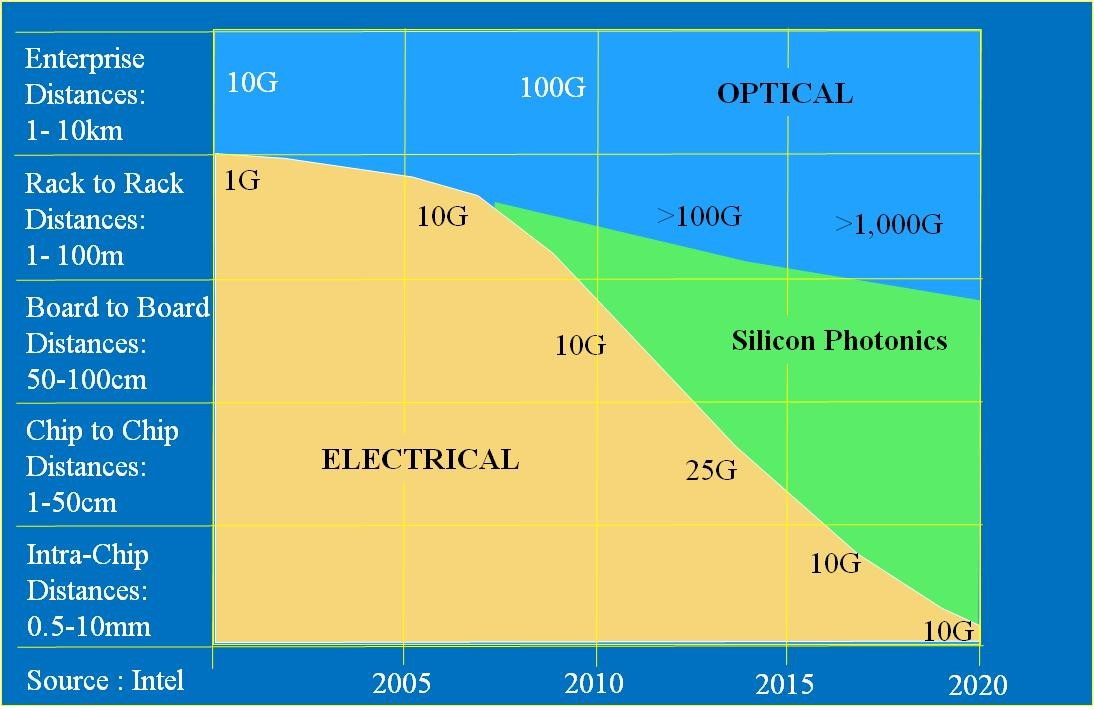
\includegraphics[width=\textwidth]{./Pictures/figure1.jpg}
	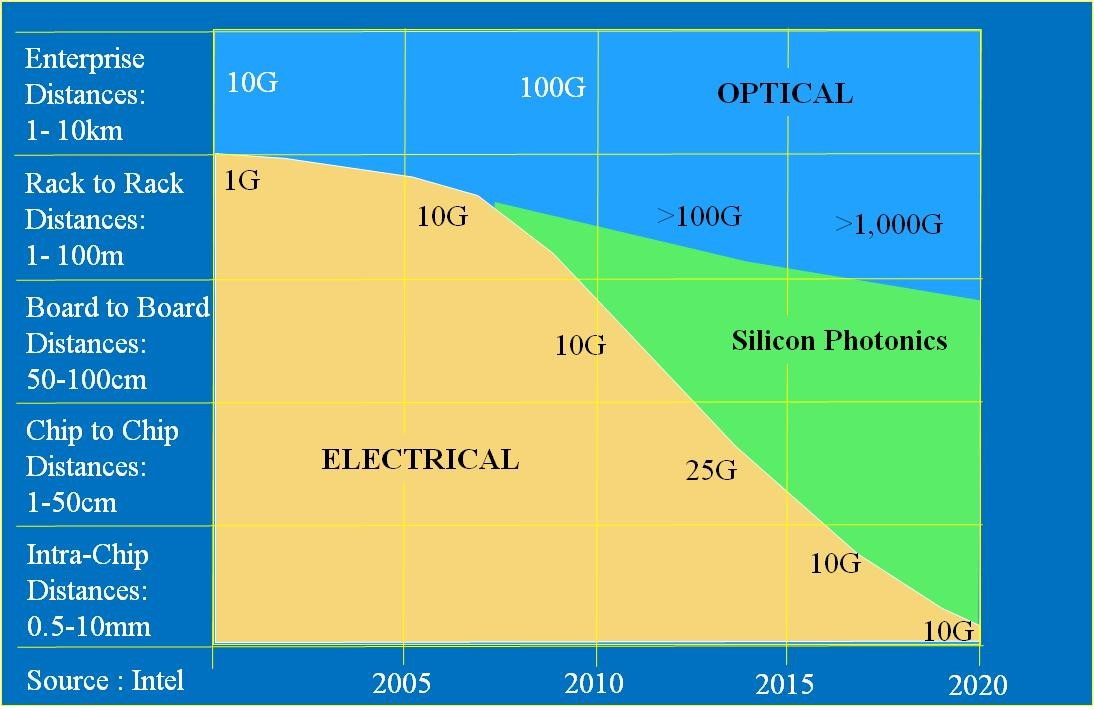
\includegraphics[width=12cm]{./Pictures/figure1.jpg}
	\caption{在不同通信距离下,电互联、硅基光通信和光纤通信的速率使用范围 \cite{Zuffada2012}}
	\label{figure1}
\end{figure}

硅基平台(Silicon-On-Insulator),即由硅衬底、二氧化硅绝缘层和硅薄膜构成的平台,不仅在传统半导体电子领域中有广泛运用,在微纳光子系统中也被广泛采用。硅基平台也成为了实现光电子集成芯片的理想平台。虽然,过去基于III-V材料的InP平台光电子平台已经实现了复杂的通信系统\cite{Meint2014an},比如片上波分复用的光收发器和多波长路由器,但是大规模应用需要价格低廉。除此之外,InP平台上的波导,垂直方向折射率差小只有1\%,导致波导的宽度和高度尺寸在工作波长量级。而硅基光波导在水平和高度方向都有将近60\%的高折射率差,因此光波导尺寸小。又因为硅基平台晶片的单位面积成本比InP晶片低,尺寸又比InP晶片大,所以硅基平台单个光器件的成本远小于InP平台。此外,硅基平台的小尺寸波导传输损耗最低达到 0.4 dB/cm \cite{Tsuyoshi2016low} 小于InP波导的最低传输损耗约为 1 dB/cm \cite{Meint2014an}。从而,硅基光电子平台越来在光通信领域受到人们的关注。

硅基光通信模块作为硅基光电子集成芯片的一个重要应用方向,其具有带宽大,功耗低,成本低的特点。图 \ref{figure1} 描述了电互联、硅基光通信和传统光纤通信和在不同距离下的适用速率范围 \cite{Zuffada2012}。图 \ref{figure1} 也预测了随着通信速率的逐年提高,硅基光通信在短距离将逐渐代替电互联。因此,硅基光集成芯片越来越受到各国的关注。美国在2004年率先提出了EPIC (Electronic and Photonic Integrated Circuits on Si)计划,研究硅基光电子集成平台,这将有助于通信,传感,微波光子学等研究方向的发展\cite{Shah2005}。欧洲在2008年提出了HELIOS (pHotonics ELectronics functional Integration on CMOS)计划,研究基于CMOS工艺的硅基光电子平台 \cite{HELIOS}。日本也紧跟而上,在2010年提出了PECST(Photonics and Electronics Convergence System Technology),推动硅基光电子平台的发展,实现芯片间的通信带宽密度达到10 Tb/s/cm\SP{2}\cite{Arakawa2013Silicon}。

光集成芯片的概念最早是由美国贝尔实验室的Miller在1969年提出来的\cite{miller1969}。随后1993, 美国空军科学研究实验室的Richard A. Soref提出了的硅基光电子集成芯片的概念\cite{Soref1993},见图 \ref{figure2} (a). 硅基光电子芯片是在同一片硅衬底上集成了负责逻辑和驱动的晶体管,负责光通信的激光器,调制器,光放大器,光探测器,光无源结构,光波导和光纤的耦合结构。在接下来的20多年内,全世界的知名高校和半导体公司都投入大量资金到这个领域中。在2011年,见图 \ref{figure2} (b), Intel厚积薄发推出了世界上第一款硅基光通信芯片包含了片上的激光器,纯硅调制器和硅锗探测器的光通信模块,实现了单通道12.5 Gbps的传输速率 \cite{Paniccia2011}。在2012年,见图 \ref{figure2} (c, d), IBM紧接发布了利用改进的90 nm CMOS工艺线,实现了在单个硅片上同时集成晶体管和的25 Gbps的光调制器和探测器 \cite{Assefa2012}。Intel虽然集成了激光器但是没能在单片上同时集成晶体管,而IBM虽然集成了晶体管,却没能集成激光器并且缺少完整光收发链路的展示。在2015年,美国伯克利大学和麻省理工大学的Chen Sun等首次展示了直接在商业化的45 nm CMOS流水线上,制作硅基光电子集成芯片 \cite{sun2015single}。该单块芯片,见图\ref{figure3} (a), 上不仅包含处理器,内存,还包含光收发模块。并且他们还展示了如图 \ref{figure3} (b) 所示的处理器的芯片和内存的芯片直接用光互联技术进行时时数据的运算和处理。虽然该硅基光电子芯片依旧缺少片上的激光器和放大器,但是该芯片是目前最复杂的单片硅基光电子芯片,包含了700万个晶体管和850个光模块。

\begin{figure}[htb]
	\centering
	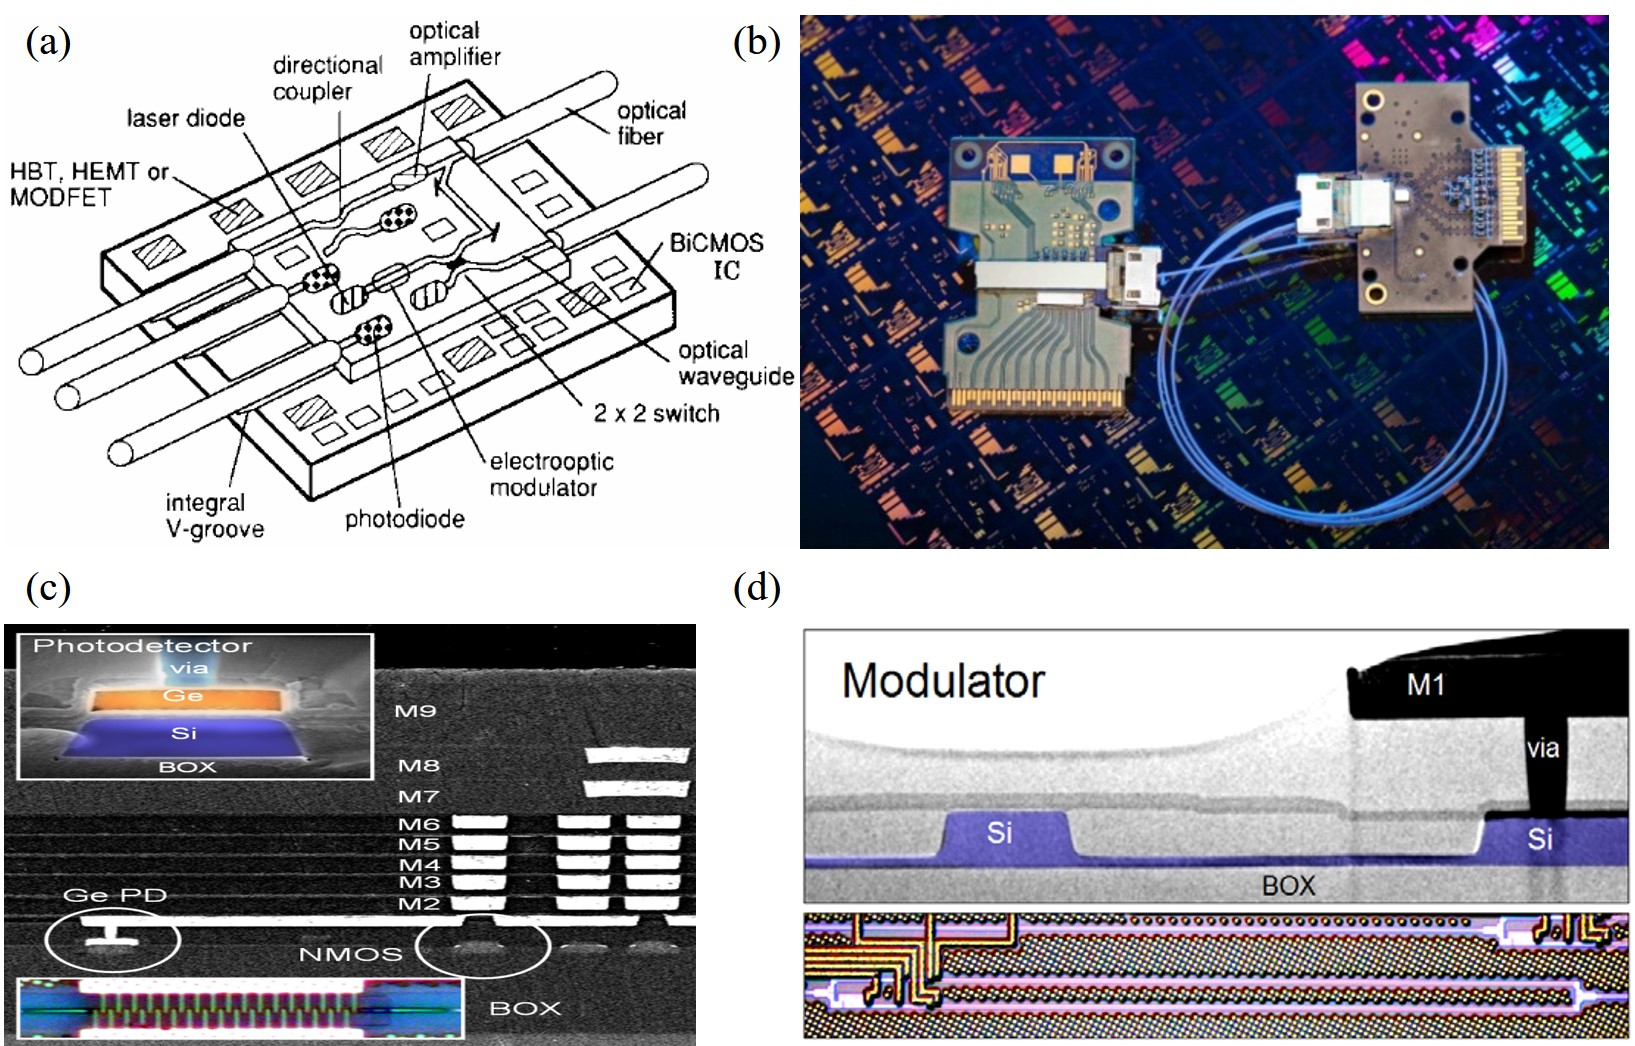
\includegraphics[width=12cm]{./Pictures/figure2.jpg}
	\caption{ (a) 最早的硅基光电子芯片概念图 \cite{Soref1993};(b)Intel的硅基光收发模块\cite{Paniccia2011};(c,d) IBM的硅基探测器和调制器\cite{Assefa2012}}
	\label{figure2}
\end{figure}

\begin{figure}[htb]
	\centering
	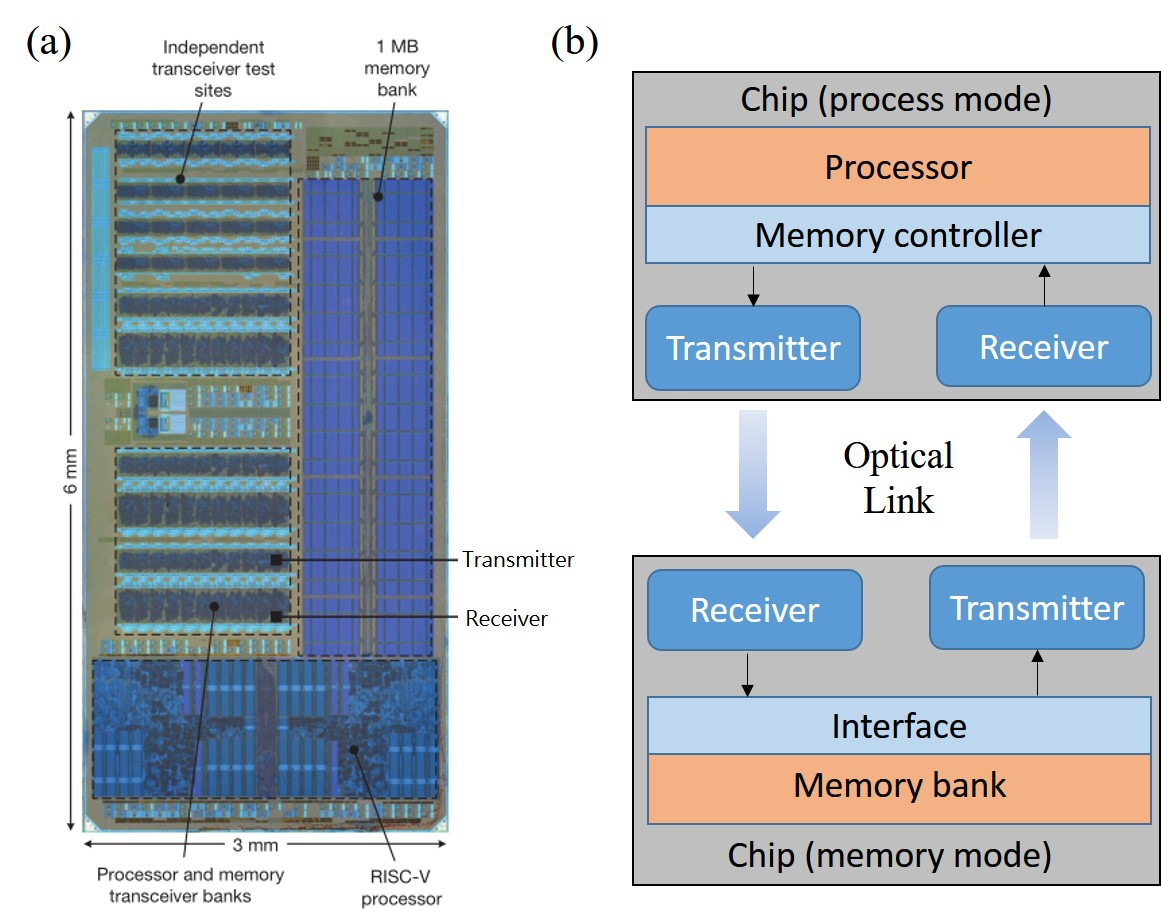
\includegraphics[width=10cm]{./Pictures/figure3.jpg}
	\caption{ (a) 单片硅基光电子芯片,包含处理器,内存,光收发模块\cite{sun2015single};(b) 处理器芯片和内存芯片间光互联示意图}
	\label{figure3}
\end{figure}

\section{硅基光调制器}
硅基光调制器做为硅基光通信模块中不可缺少的一环,用于电信号向光信号的转化,影响着光通信模块的通信速度和能耗,一直硅基光通信领域的重点和难点。虽然硅基光调制器的光学结构,电极和材料可以有很多种,但是评价硅基光调制器的性能好坏可以由以下5个指标看出:
\begin{enumerate}[(1)]
	\item 调制速率(Data Transfer Rate, BR),通常用单位时间内多少比特的信息从电信号转化为光信号来表示,单位是bps。在光调制器中调制速率一般是Gbps的数量级。描述调制器的速率还可以通过调制带宽的3 dB来表述($f$\SB{3-dB})。数字信号光调制器的电光响应频谱如同一个低通滤波器,$f$\SB{3-dB}就是调制器的电光响应降低到最大值的一半时的频率。调制器的调制速率大于调制器的调制带宽,两者的关系可以通过香农有噪信道编码定理(Shannon–Hartley theorem)联系。当没有噪声时,对于二进制编码调制速率可以达到调制带宽的两倍。
	\item 消光比(Extinction Ratio, ER)也称作调制深度,表示光在信号0和1时强度的比值,用dB表示。 消光比越高,信噪比也越好。
	\item 能耗(Energy Consumption, EC)表示将单个比特的信息从电信号转化到光信号上所消耗的电的能量。能耗的公式如下所示:
		\begin{equation}
		\label{Equ:EC}
		EC = CV_{pp}^{2}/4 + I_{average}V_{bias}/BR
		\end{equation}
	该公式分为两部分,第一部分是动态调制的能耗和第二部分是静态偏执的能耗。其中$C$是调制区域的等效电容,$V_{pp}$是驱动电压的峰峰值,$I_{average}$是直流偏置和吸收光子的而产生电流,$V_{bias}$是偏置电压,BR是调制速率。
	\item 插入损耗(Insertion Loss,IL)是调制器在全通状态下的输入光信号和输出信号的差值。插入损耗也会影响产生信号的信噪比。这些损耗包含调制器引入的反射,材料的损耗,模式不匹配引起的损耗。
	\item 器件尺寸(Footprint)是硅基光调制器光学结构加上调制区域电极结构的总尺寸。调制器的尺寸也是在硅基光调制器比较重要的参数,影响了调制器的集成度。尺寸越小的硅基光调制器在硅基光通信模块中越受到欢迎。
	\item 光学带宽(Optical bandwidth)是硅基光调制器调制波长的范围。通常谐振型的光调制器,调制波长窄,只能在谐振波长处调制。而其他类型的光调制器有比较大的光学带宽。	
\end{enumerate}

下面将讨论目前硅基光调制器在光学结构和电学结构的研究成果,概括不同材料在硅基平台上实现光调制器的最新进展。
\subsection{硅基光调制器的光学结构}
硅基光调制器如同传统的光调制器,是利用电信号改变材料折射率的实部或者虚部,从而调制器光信号的相位或者幅度。材料的折射率可以用可以表示为:
\begin{equation}
	\label{Equ:index}
	\widetilde{n(\lambda)} = n(\lambda) + j\kappa(\lambda) =  n(\lambda) + j\frac{\lambda\alpha(\lambda)}{2\pi}
\end{equation}
其中$n$为材料折射率的实部,$\kappa$为材料折射率的虚部(称作消光系数)。$\alpha$是材料单位长度的损耗。$n, \kappa, \alpha$都是和波长相关。其中$\kappa$和$\alpha$是线性关系。$n$和$\kappa$可以用通过Kramers-Kronig联系到一起\cite{o1981kramers}。

\begin{figure}[htb]
	\centering
	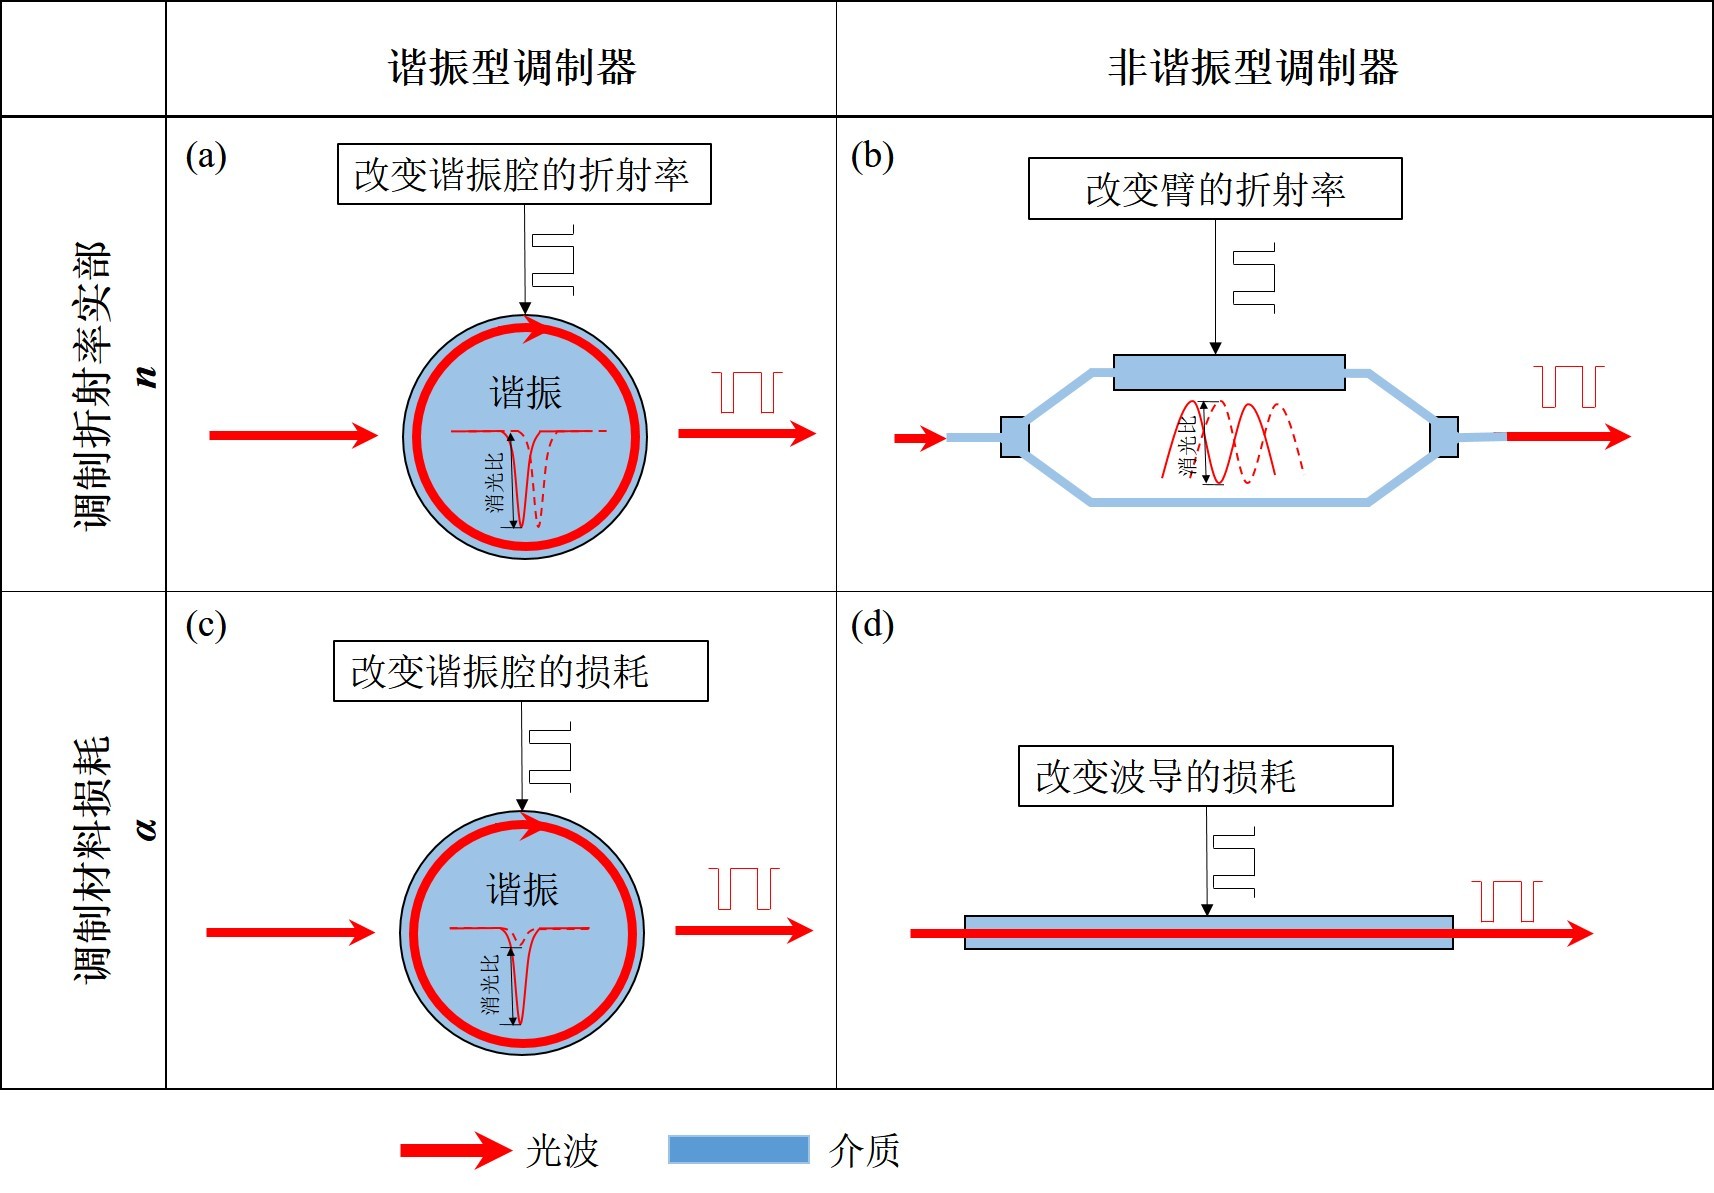
\includegraphics[width=12cm]{./Pictures/fig_mod_opt_type.jpg}
	\caption{ (a, b) 分别是通过调制折射率实部的谐振和非谐振型光调制器;(c, d)分别是通过调制材料损耗的谐振和非谐振型光调制}
	\label{fig_mod_opt_type}
\end{figure}
图 \ref{fig_mod_opt_type} 概括了硅基光调制器的光学结构的四大类型。前两类都是利用电光效应改变光的相位,再利用光学结构转化为光强度的变化。后两类是利用电吸收效应直接改变光的强度。

第一类如图\ref{fig_mod_opt_type} (a) 所示,通过调制折射率实部,改变谐振波长的位置,实现特定波长的调制。这类调制器的特点是结构紧凑,速度快,驱动电压小,能耗低。图\ref{fig_mod_opt_type_real} (a) 展示了最早利用这种结构实现的小尺寸硅基光调制器的实例\cite{xu2005micrometre}。该调制器利用载流子注入效应,调制硅波导的折射率,移动微环的谐振峰,从而实现谐振波长处光强的调制。

第二类如图\ref{fig_mod_opt_type} (b) 所示,也是通过调制折射率实部,实现相位的调制。这类调制器但是利用马赫曾德(MZI)结构,将一根波导上的相位变化,转变成强度调制器。其特点是速度快,光学带宽大。图\ref{fig_mod_opt_type_real} (b) 展示了最早利用这种结构的实现速度达到Gbps的硅基光调制器实例\cite{liu2004high}。该调制器也是利用载流子注入效应,实现马赫曾德一臂的相位变化,从而调制输出的光强。

第三类如图\ref{fig_mod_opt_type} (c)所示,通过调制微环的损耗,从而影响微环的谐振波长处的临界耦合系数,从而调制谐振波长的强度。这类调制器的特点是结构紧凑,驱动电压低,能耗低,速度快。图\ref{fig_mod_opt_type_real} (c) 展示了最早利用这种结构的硅基光调制器的实施方案\cite{Midrio2012graphene}。该调制器利用微环中部分硅波导上的石墨烯,调制石墨烯的损耗,导致微环损耗的变化,从而调制谐振波长处光的强度。由于这类调制器是最近2012年才提出的,目前只在氮化硅平台上有实例\cite{phare2015graphene},在硅基平台上没有实例,只有理论分析的结果\cite{Midrio2012graphene}。

第四类如图\ref{fig_mod_opt_type} (d)所示,直接通过改变波导的损耗,实现光强度的调制。这类调制器的特点是结构紧凑,能耗低,速度快,光学带宽大。图\ref{fig_mod_opt_type_real} (d) 展示了利用这种结构的硅基光调制器实例\cite{tang201150}。该调制器是将InP混合集成到硅波导上,再利用InP多量子阱材料(Multiple Quantum Well, MQW)中量子束缚Stark效应(Quantum Confined Stark Effect, QCSE)实现在不同电压下,材料吸收峰的移动,导致波导的损耗的变化,从而实现光强度的变化。

这四类调制器中的马赫曾德结构除了能用于将光的相位变化转变成强度变化外,还经常被用于高级调制码型的发生器,比如文献[\citenum{Dong2012coherent}]中就利用马赫曾德结构实现正交相移键控(Quadrature Phase-Shift Keying, QPSK)调制码形,并且结合了偏振复用,使单通道的调制速度提高到112 Gbps。
\begin{figure}[htb]
	\centering
	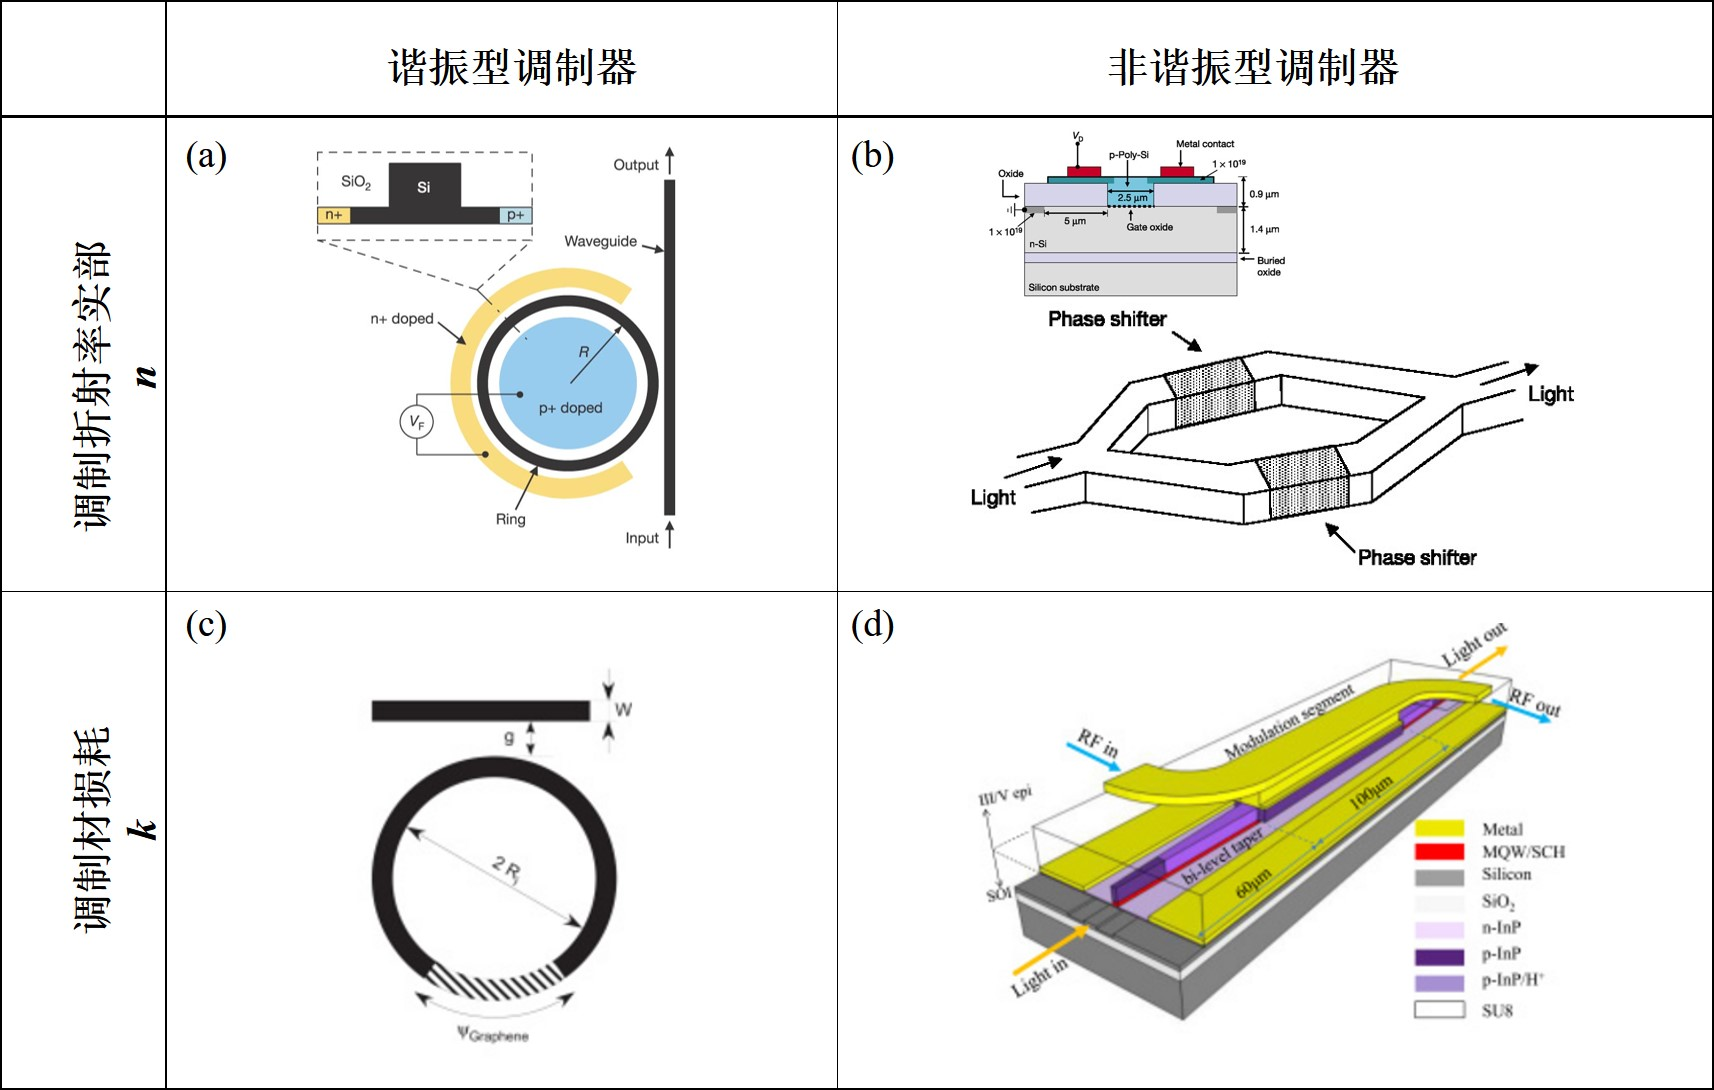
\includegraphics[width=12cm]{./Pictures/fig_mod_opt_type_real.jpg}
	\caption{ (a, b) 分别是通过调制折射率实部的谐振和非谐振型光调制器的实例\cite{xu2005micrometre,liu2004high};(c, d)分别是通过调制材料损耗的谐振和非谐振型光调制的实例\cite{Midrio2012graphene,tang201150}}
	\label{fig_mod_opt_type_real}
\end{figure}

\subsection{硅基光调制器的电极结构}
硅基光调制器的电极结构对调制速率和能耗也有很大影响。图\ref{fig_mod_ele_type}展示了目前硅基光调制器所有的四种电极结构。这四种电极结构已经在InP光调制器和LiNbO\SB{3}光调制器上被广泛应用。下面将讨论这四种电极结构特点。

\begin{figure}[htb]
	\centering
	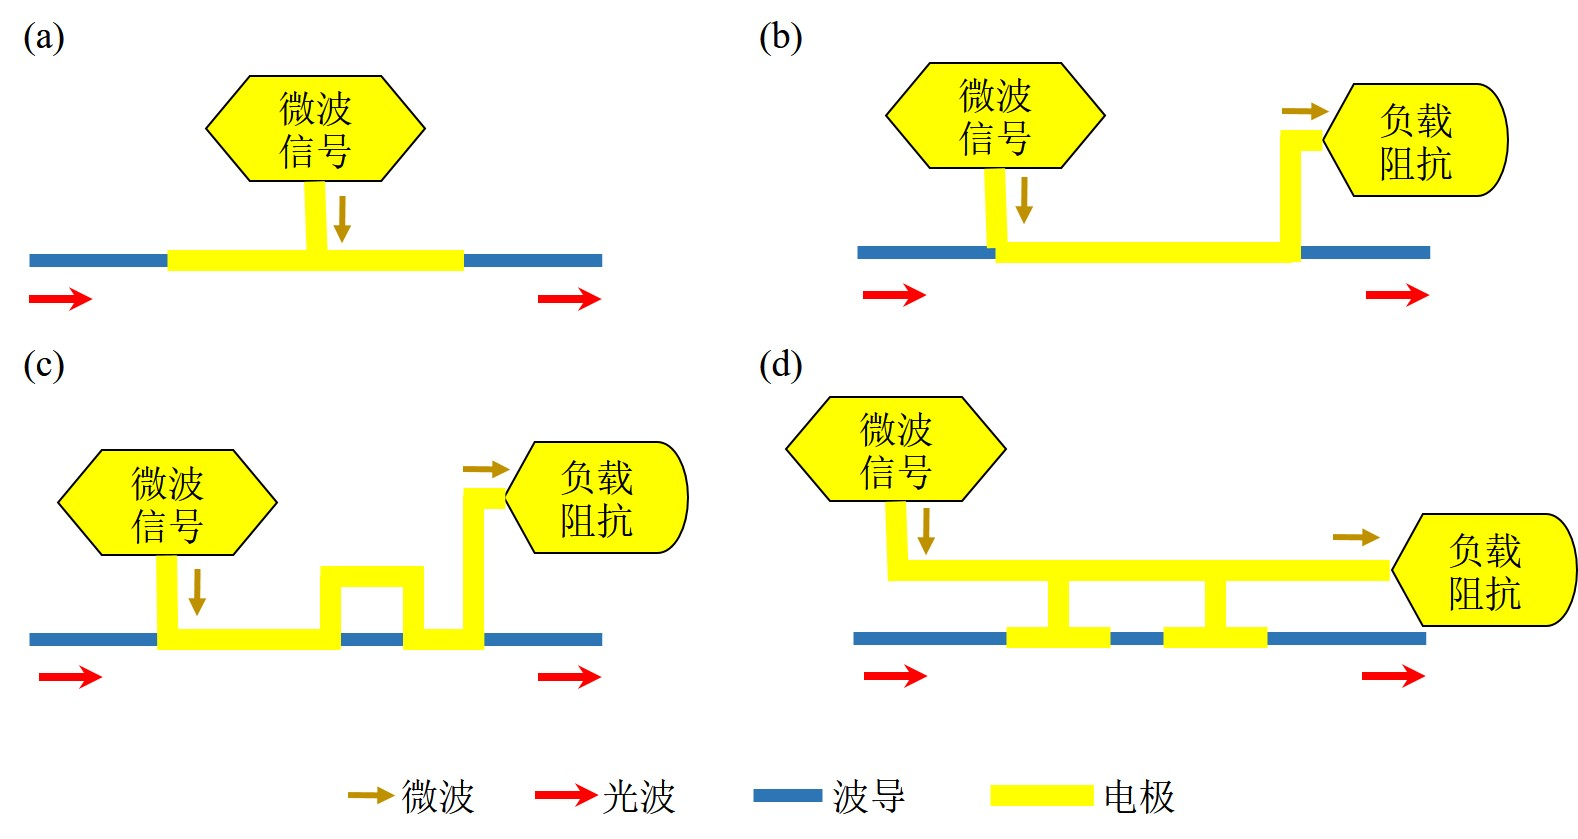
\includegraphics[width=12cm]{./Pictures/fig_mod_ele_type.jpg}
	\caption{ (a) 集总电极;(b)行波电极;(c)分段传输线电极;(d)电容负载行波电极}
	\label{fig_mod_ele_type}
\end{figure}

第一种电极称为集总电极(Lumped Electrode, LE)如图\ref{fig_mod_ele_type} (a)所示, 这种电极在调制区域的长度小于100 $\mu m$的硅基光调制器中被广泛使用,尤其是小型的谐振型硅基光调制器。由于这类电极末端没有负载是开路,导致微波信号末端反射,集总电极上成为驻波,从而降低所需外界的调制电压,同时也避免了偏置电压在负载上损失的能耗。因此,集总电极在小尺寸,低驱动电压,低能耗的电极上有广泛的应用。图\ref{fig_mod_ele_type_real} (a)展示了集总电极用于InP混合集成到硅波导上的调制器\cite{tang2012energy},实现了低能耗,低驱动电压,小尺寸的调制器。

第二中电极称为行波电极(Traveling Wave Electrode, TWE)如图\ref{fig_mod_ele_type} (b)所示,这种电极在调制区域大于100 $\mu m$的硅基调制器中被广泛使用,尤其是马赫曾德的硅基光调制器。由于这行波电极调制器需要将电极考虑成为传输线,因此需要设计电极本征阻抗与标准的微波器件的本征阻抗50 $\Omega$相匹配,并且使传输线的传播常数和波导中光的传播常数相匹配,从而尽可能提高调制器的调制带宽。因此,使用行波电极的调制器调制速度高于集总电极的调制器,但是在尺寸,驱动电压,能耗上差于集总电极的调制器。图\ref{fig_mod_ele_type_real} (b)展示了行波电极用于InP混合集成到硅波导上的调制器\cite{tang2012energy},实现了高速的硅基光调制器。

第三种电极称为分段传输线电极(Segmented Transmission Line Electrode, STLE)如图\ref{fig_mod_ele_type} (c)所示, 这种电极也是主要用于调制长度大于100 $\mu m$以上,并且电极的本征电阻和50 $\Omega$相差大,或者微波和光波的传播常数相差较大的硅基光调制器。分段传输线电极是行波电极的一个更为普遍的形式,相比行波电极,其调制带宽可以进一步提高,但是能耗不会有所减少,而尺寸将更进一步增大,。图\ref{fig_mod_ele_type_real} (c)展示了分段传输线电极用于InP混合集成到硅波导上的调制器\cite{tang2012energy},实现了目前调制速度最快的硅基光调制器。

第四种电极称为电容负载行波电极(Capacitively-Loaded Traveling-Wave Electrode, CLTWE)如图\ref{fig_mod_ele_type} (d)所示, 这种电极在硅基光调制器中的应用比较少,主要用于调制长度大于500 $\mu m$以上,并且电极的本征电阻和50 $\Omega$相差大,或者微波和光波的传播常数相差较大的硅基光调制器。由于电容负载行波电极整体和如同行波电极一样,但在单个周期内,调制器区域是集总电极,因此这类电极用于兼顾传输速度和低驱动电压。不过,由于在单个调制器区域还有没参与调制的电极,因此电容负载行波电极的尺寸比较大。图\ref{fig_mod_ele_type_real} (d)展示了电容负载行波电极用于InP混合集成到硅波导上的调制器\cite{tang2012energy},实现了马赫曾德的光调制器。

这四种电极各有优缺点,如果需要尺寸小,能耗低的调制器,可以采用集总电极。如果需要尽可能高的调制速度,或者调制器区域长度比较长时则可以采用行波电极或分段传输线电极结构。而电容负载行波电极是集总电极和分段传输线折中的形式,可以在这两种电极都无法满足要求的情况下使用。
\begin{figure}[htb]
	\centering
	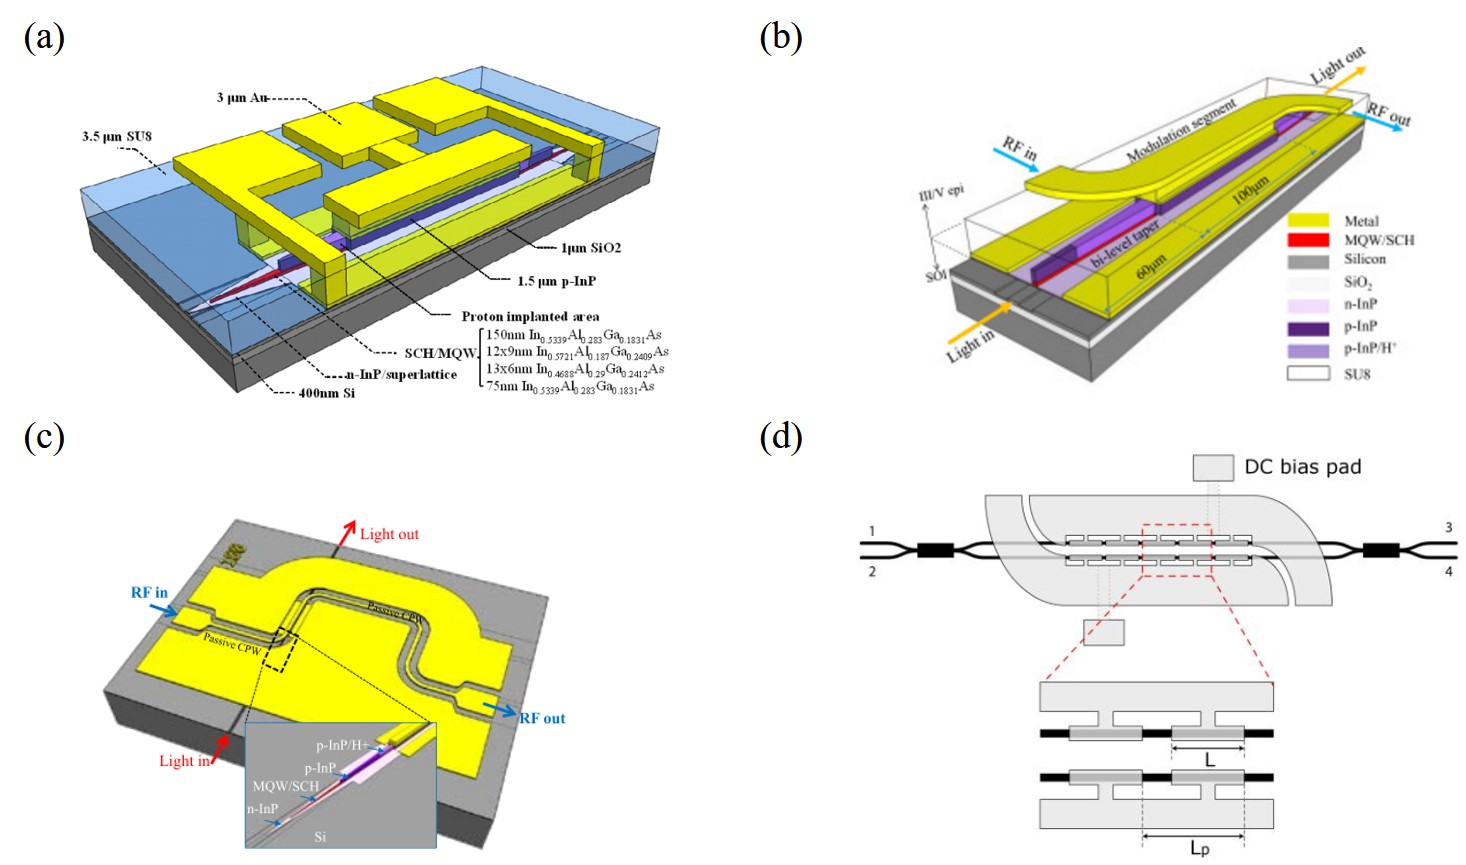
\includegraphics[width=12cm]{./Pictures/fig_mod_ele_type_real.jpg}
	\caption{ (a) 集总电极的实例\cite{tang2012energy};(b)行波电极实例\cite{tang201150};(c)分段传输线电极实例\cite{tang2012over};(d)电容负载行波电极实例\cite{chen2011forty}}
	\label{fig_mod_ele_type_real}
\end{figure}
\subsection{纯硅基光调制器}
纯硅的光调制器可以与标准的半导体工艺完美结合,满足实际调制器小尺寸,低功耗或者高速,大光学带宽的需求,而且调制器的加工成本低。因此,纯硅硅光调制器一直是硅基光调制器中最热门的研究方向。不过由于硅是反演中心对称的晶体,导致它不具有线性电光效应,即Pockels效应,并且在通信1.3 $\mu m$ 和 1.55 $\mu m$处,二阶非线性Kerr也很弱\cite{soref1987electrooptical}。虽然硅的热光系数很大,但是热光效应作为光调制器速度太慢\cite{cocorullo1992thermo}。

目前,纯硅基光调制器采用的是等离子色散效应(plasma dispersion effect)实现速度达到Gbps以上的光调制器。硅基光调制器采用三种方式实现等离子色散效应,分别是载流子注入(Carrier injection),载流子聚集(Carrier accumulation)和载流子耗尽(Carrier depletion)。

载流子注入的实现方式是最早被提出来的,但是靠这种方式的调制器速度由硅中少数载流子寿命决定。目前载流子注入的光调制器速度最多达到Gbps,通过预加重(pre-emphasis)的特殊码形速度目前最高达到18 Gbps\cite{manipatruni2007high}。

载流子聚集对的方式是最早实现高于1 Gpbs的纯硅基光调制器。载流子聚集调制器是通过将自由载流子聚集到波导中的薄介质层附近从而实现改变折射率。因此,载流子聚集的调制器速度突破了少数载流子寿命的约束,调制速度由等效电容和电阻决定速率。由于薄介质层的厚度薄,载流子聚集效率低,等效电容大,从而影响了最高的速度,目前载流子聚集的光调制器最快达到25 Gbps\cite{fujikata201025}。

载流子耗尽的方式是目前实现最快硅基光调制器。载流子耗尽调制器是通过外界反向偏压,控制波导中耗尽区和光场相互作用的面积从而实现调制。因此,载流子耗尽的调制器也突破了载流子寿命的约束,调制速度也由等效电容和电阻决定速率。由于耗尽区的宽度可以通过本pn结的掺杂浓度,或者pin结构中i层的厚度,或者反向偏压的大小控制,因此等效电容可以方便的根据实际所需速率设计。目前载流子耗尽的光调制器最快速度达到了60 Gbps\cite{Xiao201360}。

由于纯硅基调制器和半导体工艺完美结合,因此大学实验室只能提供设计,然后提交给拥有完全流水线的半导体代工公司(比如比利时的Imec-ePIXfab \cite{Imec, absil2015silicon}、新加坡的OpSIS-IME \cite{novack201330}、美国的IBM的45nm的SOI半导体流水线\cite{narasimha2006high}等)生产制作。另外,中国的中芯国际(Semiconductor Manufacturing International Corporation, SMIC)也提供硅调制器的加工\cite{xu2012high,xiao2013high,Xiao201360}。表\ref{sil_mod}总结了近期纯硅基光调制器方面的最好的结果。目前纯硅基光调制器的最高调制速度达到了60 Gbps,能耗最低能到0.1 fJ/bit,驱动电压最低需要50 mV。

{
	\begin{table}[htb]
		\zihao{5}
		\caption{比较近期纯硅基光调制器的性能。PhC: 光子晶体;Ring:微环; Zigzag:锯齿;Disk:微盘;MZI:马赫曾德}
		\label{sil_mod}
		\centering
		\begin{tabular}[t]{p{1.5cm}ccp{1.2cm}ccccccc}
			\hline
			掺杂方式 & 光学结构 & 电极结构 & 调制区尺寸 & 调制速度 & 动态能耗 & 消光比 & 插入损耗 & 调制电压\\
			\hline
			lateral pn \cite{xiao2013high,Xiao201360} & MZI & TW  & 750 $\mu m$ & 60 Gbps & - & 4.4 dB & 2.0 dB& 6.5 V\\
			zigzag pn\cite{Xiao201360} & Ring & LE & 22 $\mu m$ & 60 Gbps & - & 4.2 dB & - & 6 V\\
			vertical pn\cite{timurdogan2014ultralow} & Disk & LE & 4.8 $\mu m$ & 44 Gbps & 17.4 fJ/bit & 8.0 dB & 0.92 dB & 2.2 V\\
			lateral pin\cite{shakoor2014ultra} & PhC & LE & ~6.0 $\mu m$ & 1 Gbps & 0.1 fJ/bit & 2.0 dB & - & 50 mV\\			
			lateral pn\cite{Pantouvaki201556} & Ring & LE & 10 $\mu m$ & 56 Gbps & 45 fJ/bit & 4.0 dB & 3.0 dB& 2.5 V\\
			lateral pipin\cite{Ziebell201240} & MZI & TW & 950 $\mu m$ & 40 Gbps & - & 3.2 dB & 2.5 dB & 6 V \\
			lateral pin\cite{Baba201350} & Ring & LE & 20 $\mu m$ & 50 Gbps & - & 4.6 dB & 5.2 dB & 1.96 V\\
			lateral pn\cite{Ding2013electro} & MZI & TW & 2 $mm$ & 40 Gbps & 32.4 fJ/bit & 3.5 dB & 12.5 dB & 0.36 V\\
			\hline
		\end{tabular}
	\end{table}
}

纯硅基光调制器波导的掺杂方式根据不同等离子色散实现方式分有很多种\cite{reed2010silicon},在此主要介绍三种常用且特色的方案,如图\ref{fig_silicon_mod_cross}所示。表\ref{sil_mod}也展示不同掺杂方式的硅基光调制器最新最好的性能。
第一种是水平掺杂的pn结或者pin结,如图\ref{fig_silicon_mod_cross}(a)所示。这种掺杂方式使用最为广泛,用于目前调制速度达到60 Gbps的纯硅基MZI光调制器(如图\ref{fig_silicon_mod}(a)所示)\cite{xiao2013high}。另外,驱动电压只有50 mV 并且能耗只有0.1 fJ/bit的光子晶体(Photonic Crystal, PhC)结构的纯硅基光调制器(如图\ref{fig_silicon_mod}(b)所示)也是采用了水平掺杂的pn结\cite{,shakoor2014ultra}。
第二种是交趾掺杂和其改进型的锯齿掺杂,如图\ref{fig_silicon_mod_cross}(b)所示。这种掺杂方式目前主要用于提高单位长度的调制效率,目前调制速度最快达到60 Gbps的纯硅基微环光调制器(如图\ref{fig_silicon_mod}(c)所示)就是采用这种结构\cite{Xiao201360}。
第三种是在2014年才提出的垂直方向pn结,如图\ref{fig_silicon_mod_cross}(c)所示。通过种掺杂方式,并且结合微盘结构(如图\ref{fig_silicon_mod_cross}(c)所示),具有pn掺杂谐振型光调制器中最高的电光效应,达到了250 pm/V,这是之前的十倍\cite{timurdogan2014ultralow}。

\begin{figure}[htb]
	\centering
	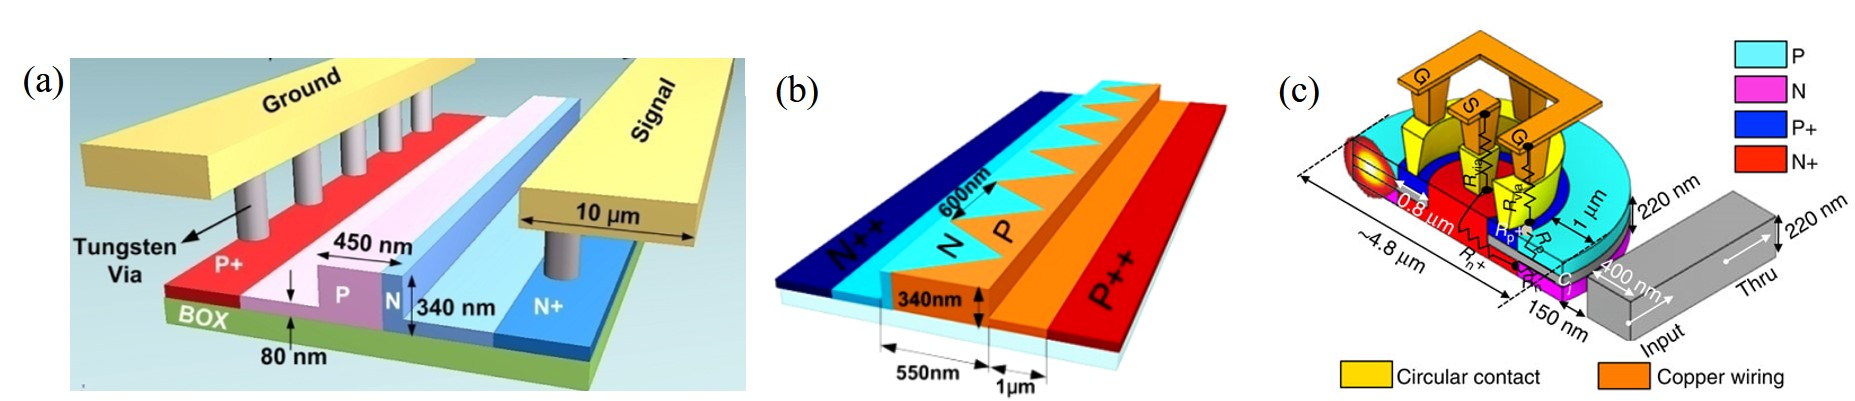
\includegraphics[width=15cm]{./Pictures/fig_silicon_mod_cross.jpg}
	\caption{ (a) 中心偏移的水平pn结\cite{xiao2013high};(b)齿状交趾的纵向pn结\cite{Xiao201360};(c)垂直方向的pn结\cite{timurdogan2014ultralow}}
	\label{fig_silicon_mod_cross}
\end{figure}

\begin{figure}[htb]
	\centering
	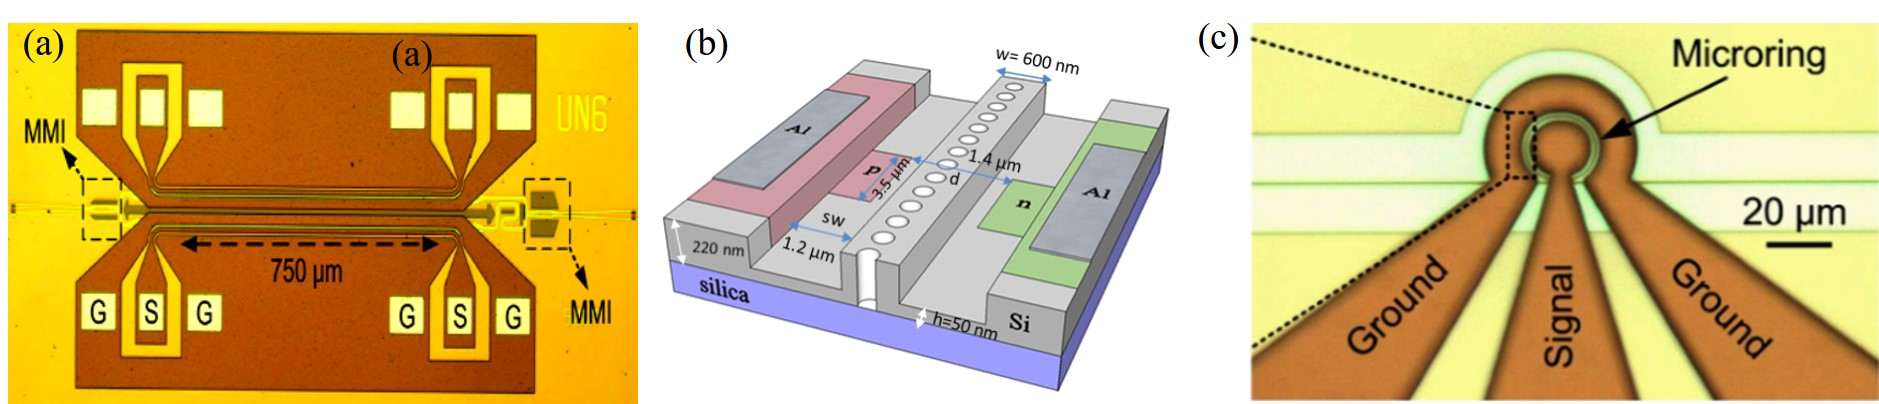
\includegraphics[width=15cm]{./Pictures/fig_silicon_mod.jpg}
	\caption{ (a) 60 Gbps的MZI纯硅基光调制器\cite{Xiao201360};(b)能耗0.1 fJ/bit的光子晶体纯硅基光调制器\cite{shakoor2014ultra};(c) 60 Gbps的锯齿掺杂微环纯硅基光调制器\cite{Xiao201360}}
	\label{fig_silicon_mod}
\end{figure}
\subsection{硅基外延锗硅光调制器}
为了克服纯硅基是间接带隙对的半导体,没有电吸收效应的缺点,因此需要将其他材料和硅集成实现光调制器。锗材料具有直接带隙半导体基于Franz-Keldysh现象的电吸收效应\cite{frova1965franz},并且锗材料也是如今CMOS工艺的标准材料,因此硅基外延锗硅(GeSi)光调制器成为了一个热门的研究方向。最早实现GeSi光调制器是2008年\cite{liu2008waveguide},研究人员通过在硅上先生长一层仅40 nm的GeSi缓冲层,在高温生长在Ge中掺有少量Si的GeSi材料,最后高温退火减少材料中的缺陷。除此之外,研究人员虽然在2005年,实现了硅上生长GeSi多量子阱结构并且发现了多量子阱中量子束缚Stark效应(Quantum Confined Stark Effect, QCSE)\cite{kuo2005strong},但是,研究人员在2010年,才实验展示了基于硅基GeSi多量子阱结构QCSE的电吸收调制器\cite{rong2010quantum}。表\ref{sil_ge_mod}展示了目前不同GeSi材料下的硅基外延锗光调制器的最佳工作性能。
{
	\begin{table}[htb]
		\zihao{5}
		\caption{近期硅基外延锗硅光调制器的最佳性能。FK:Franz-Keldysh;}
		\label{sil_ge_mod}
		\centering
		\begin{tabular}[t]{p{1.5cm}ccp{1.2cm}ccccccc}
			\hline
			调制原理 & 工作波长 & 电极结构 & 调制区尺寸 & 调制速度 & 动态能耗 & 消光比 & 插入损耗 & 调制电压\\
			\hline
			Ge FK\cite{Srinivasan201656} & 1615 nm & LE  & 40 $\mu m$ & 56 Gbps & 12.8 fJ/bit & 4.6 dB & 4.9 dB& 2 V\\
			GeSi FK\cite{Dazeng2013high} & 1550 nm & LE  & 50 $\mu m$ & 28 Gbps & 147 fJ/bit & 5.9 dB & 4.8 dB& 3 V\\
			Ge/GeSi QCSE\cite{chaisakul201223} & 1448 nm & LE & 90 $\mu m$ & 23 GHz & 108 fJ/bit & - & - & 1V\\
			\hline
		\end{tabular}
	\end{table}
}

从表\ref{sil_ge_mod}可以看出,目前调制速度最快(56 Gbps)和能耗最低(12.8 fJ/bit)的都是基于纯锗Franz-Keldysh现象的光调制器,其结构如图\ref{fig_ge_mod}(a)所示。它的尺寸和速度都可以与纯硅基微环光调制器相媲美,并且硅基锗的光调制器光学带宽大于22nm高于纯硅基微环光调制器\cite{Srinivasan201656}。不过,纯锗的光调制器工作波长是1615 nm附件,而合理配比Ge和Si的材料的组分能将工作波长移到1550 nm。目前硅基GeSi的光调制器速度达到28 Gbps依旧有提升的空间\cite{Dazeng2013high},结构如图\ref{fig_ge_mod}(b)。另外,由于基于Ge/GeSi 多量子阱结构光调制的也能调整工作波长,但是由于这种外延结构制作最为困难,外延结构如图\ref{fig_ge_mod}(c)所示,因此发展的比较缓慢。目前它在模拟信号下最快的调制速度只有23 GHz,工作波长是1448 nm。因此,硅基外延锗的光调制器仍需要继续研究,从而实现在通信波长1.55 $\mu m$处的高速,低功耗的光调制器。除此之外,由于硅波导和锗硅调制器的材料不同,波导结构尺寸不同,因此为了实现单片集成,任需要设计硅波导到锗硅调制器的光学耦合结构。目前采用的是通过硅波导的宽度渐变的锥形结构和硅锗波导进行端面耦合,如图\ref{fig_ge_mod}(d)所示。

\begin{figure}[htb]
	\centering
	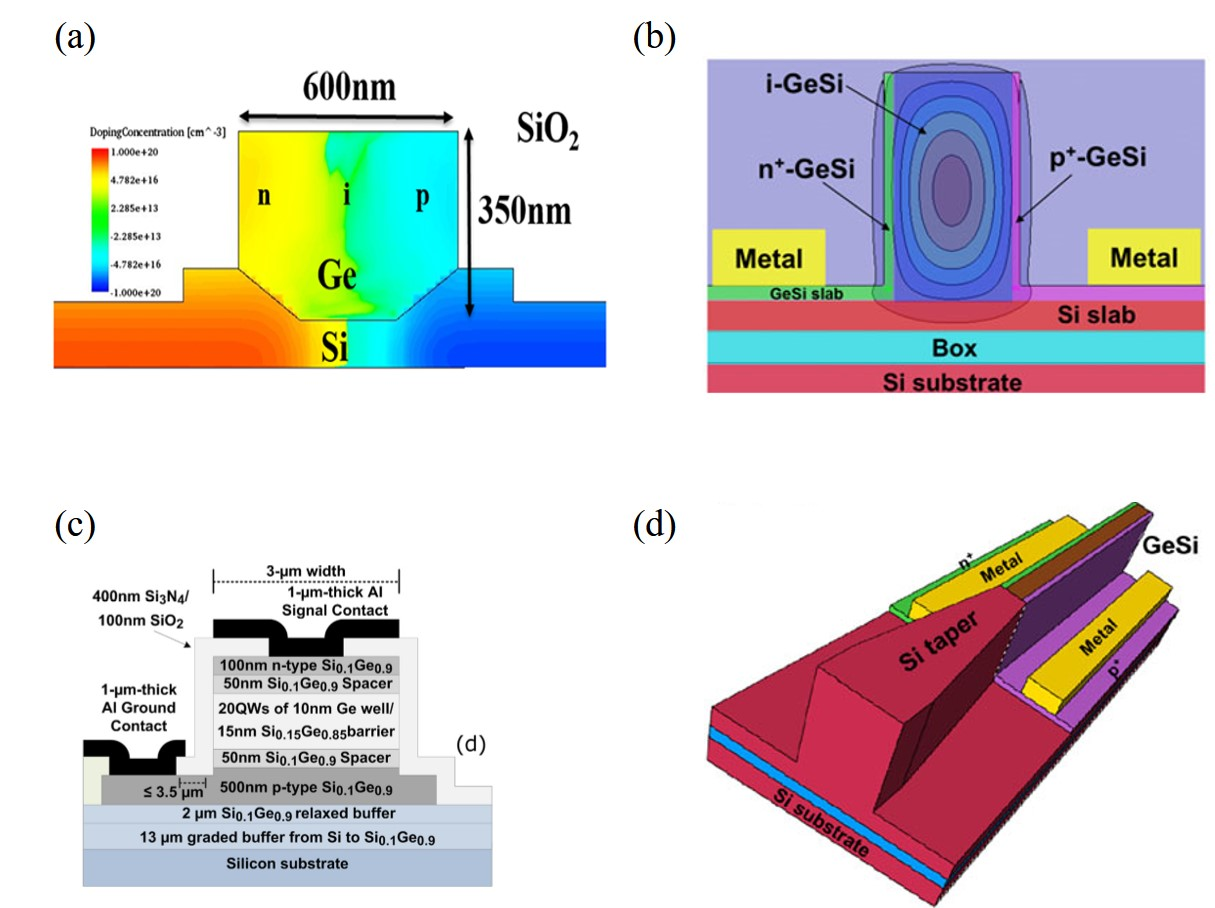
\includegraphics[width=12cm]{./Pictures/fig_ge_mod.jpg}
	\caption{ (a) 硅基锗光调制器\cite{Srinivasan201656};(b)硅基锗硅光调制器\cite{Dazeng2013high};(c)硅基锗硅多量子阱光调制器\cite{chaisakul201223};(d)硅波导和锗硅光调制器的耦合结构\cite{Dazeng2013high}}
	\label{fig_ge_mod}
\end{figure}
\subsection{硅基石墨烯光调制器}
石墨烯自从2004年被英国的研究人员发现\cite{novoselov2004electric},就在各个领域内被广泛应用。硅基石墨烯光调制器首次由是美国伯克利大学张翔小组实现,结构如图\ref{sil_graphene_mod}(a)所示,实现了小信号的3dB调制带宽达到了1.2 GHz.虽然首次展示的硅基石墨烯光调制器的速度受到器件的电容和电阻制约,但是石墨烯光调制器具有结构紧凑(40 $\mu m$),插入损耗低(2.4 dB),光学带宽大(>180 nm)的特点。随后很多研究人员,投入到高速石墨烯光调制器的研究中。
{
	\begin{table}[htb]
		\zihao{5}
		\caption{硅基石墨烯光调制器。EAM: Electro-absorption Modulator;EOM:Electro-optic Modulator;Term:Terminates}
		\label{sil_graphene_mod}
		\centering
		\begin{tabular}[t]{p{1.5cm}cp{0.8cm}p{1.2cm}ccccc}
			\hline
			调制原理 & 光学带宽 & 电极结构 & 调制区尺寸 & 调制速度 & 动态能耗 & 消光比 & 插入损耗 & 调制电压\\
			\hline
			Graphene EAM\cite{liu2011graphene} & >180 nm & LE  & 40 $\mu m$ & 1.2 GHz & - & 2.4 dB & - & 3 V\\
			Graphene EAM\cite{liu2012double} & -  & LE  & 40 $\mu m$ & 1 GHz & 1 pJ/bit & 6.5 dB & 4 dB & 3 V\\
			Graphene EAM\cite{hu2014broadband} & >80 nm & LE  & 50 $\mu m$ & 10 Gbps & 350 fJ/bit & 2.5 dB & 4 dB& 2.5 V\\
			Graphene Ring\cite{phare2015graphene} & - & LE (Term) & 30 $\mu m$ & 22 Gbps & 800 fJ/bit & - & -14 dB & 7.5 V\\
			\hline
		\end{tabular}
	\end{table}
}

表\ref{sil_graphene_mod}展示具有代表性的硅基石墨烯光调制器。双层石墨烯调制器,如图\ref{sil_graphene_mod}(b)所示,增加了光与石墨烯的相互作用,提高了的石墨烯光调制器的调制深度。随后,比利时的Imec提出的如图\ref{sil_graphene_mod}(c)所示的硅基石墨烯光调制器,通过合理设计硅波导的掺杂浓度和尺寸,以及石墨烯的和硅之间间隔,将调制器的调制速度提高到了10 Gbps\cite{liu2011graphene, hu2016broadband}。最近美国康奈尔大学的Lipson小组利用石墨烯调制微环的损耗从而影响微环的临界耦合系数,而微环的透射谱对临界耦合系数很敏感,进而实现30 GHz的石墨烯光调制器,结构如图\ref{sil_graphene_mod}(d)所示。该石墨烯的光调制器虽然制作于氮化硅的衬底,但是这种结构也可以应用于未来的高速硅基石墨烯光调制器。

\begin{figure}[htb]
	\centering
	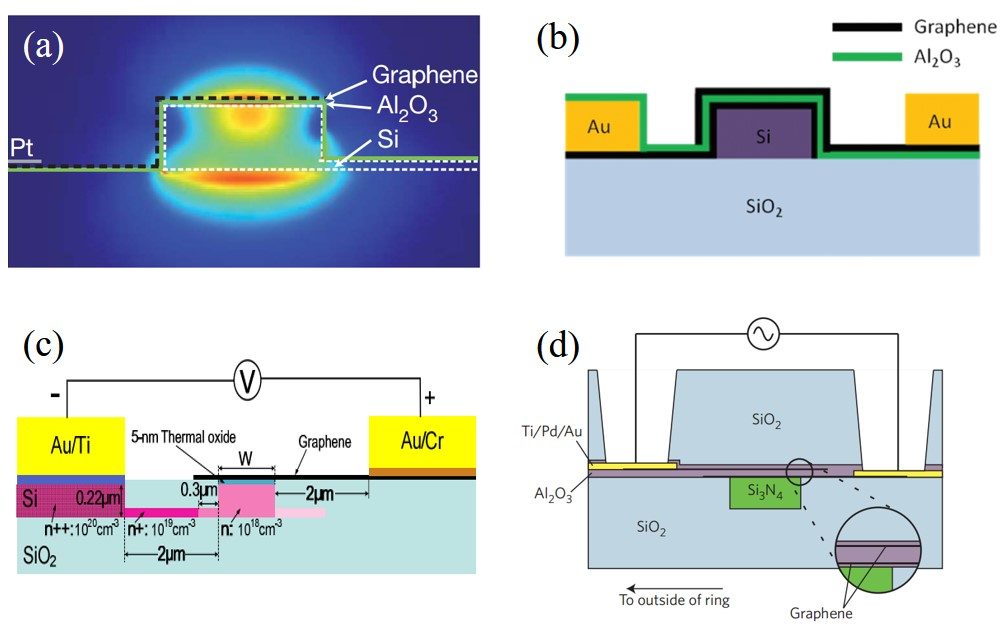
\includegraphics[width=12cm]{./Pictures/fig_graphene_mod.jpg}
	\caption{ (a) 硅基单层石墨烯光调制器\cite{liu2011graphene};(b)硅基双层石墨烯光调制器\cite{liu2012double};(c)硅基单层石墨烯光调制器\cite{hu2014broadband, hu2016broadband};(d)氮化硅基石墨烯光调制器\cite{phare2015graphene}}
	\label{fig_ge_mod}
\end{figure}

\subsection{硅基聚合物光调制器}
聚合物光调制器一直是研究的热点。目前世界上所有平台中的光调制器,调制速度最快的就是基于聚合物的光调制器。这个光调制速是在2002年由美国贝尔实验室实现的,调制带宽达到了1.6 THz\cite{lee2002broadband}。目前世界上硅基平台上的所有光调制器,调制速度最快的并且调制区域尺寸最小的也是基于聚合物的光调制器。这个光调制器是在2015年由瑞士苏黎世理工实现的,利用表面等离子体槽型波导,将光约束到纳米尺度,调制器的微波小信号3 dB带宽大于70 GHz,调制速度达到了72 Gbps,调制区域的尺寸只有6  $\mu m$。 聚合物除了速度快,其电光系数也很高,达到了230 pm/V \cite{palmer2014high},这与目前最好的纯硅光调制器的电光系数250 pm/V \cite{timurdogan2014ultralow}相当。
{
	\begin{table}[htb]
		\zihao{5}
		\caption{硅基聚合物光调制器。MZM:  Mach–Zehnder modulator;SOH: Silicon-Organic Hybrid Modulator}
		\label{sil_polymer_mod}
		\centering
		\begin{tabular}[t]{p{1.5cm}cp{1.2cm}ccccccc}
			\hline
			调制原理 & 电极结构 & 调制区尺寸 & 调制速度 & 动态能耗 & 消光比 & 插入损耗 & 调制电压\\
			\hline
			SOH\cite{palmer2014high} & LE  & 0.25 $mm$ & 40 Gbps & 420 fJ/bit & 9 dB & 6 dB & 2.1 V\\
			SOH\cite{palmer2014high} & TW  & 1.0 $mm$ & 40 Gbps & - & 8.9 dB & 6 dB & 1.5 V\\	
			SOH\cite{koeber2015femtojoule} & LE  & 1.0 $mm$ & 12.5 Gbps & 0.7 fJ/bit & -B & 6 dB & 1.5 V\\			
			Plamonic MZM\cite{haffner2015all} & LE  & 6 $\mu m$ & 72 Gbps & 25 fJ/bit & - & 8 dB & 6 V\\
			\hline
		\end{tabular}
	\end{table}
}
表\ref{sil_polymer_mod}展示了最近硅基聚合物光调制器的性能。传统的硅基聚合物光调制器是用槽型波导\cite{almeida2004guiding},将大部分光强约束到中间的聚合物中,如图\ref{fig_polymer_mod}(a)所示\cite{palmer2014high,liu2015recent}。传统的硅基聚合物光调制器利用MZI结构,如图\ref{fig_polymer_mod}(b)所示,速度能达到了40 Gbps。这类光调制器能耗最低达到0.7 fJ/bit.而最近采用表面等离子体槽型槽型波导结构,将调制器的尺寸从$10^3 \mu m$量级缩小到$\mu m$量级,速度也提高到了72 Gbps(受到测试仪器的带宽限制)\cite{haffner2015all}。这种调制器的器件结构和波导界面模场分布如图\ref{fig_polymer_mod}(c, d)所示。目前这种调制器阵列也被制作出来,展示了 4 $\times$ 36 Gbps的发射阵列\cite{heni2015high}。不过,硅基基于表面等离子体槽型波导的聚合物光调制器仍然需要进一步降低能耗,降低驱动电压,提高这类调制器的竞争力。
\begin{figure}[htb]
	\centering
	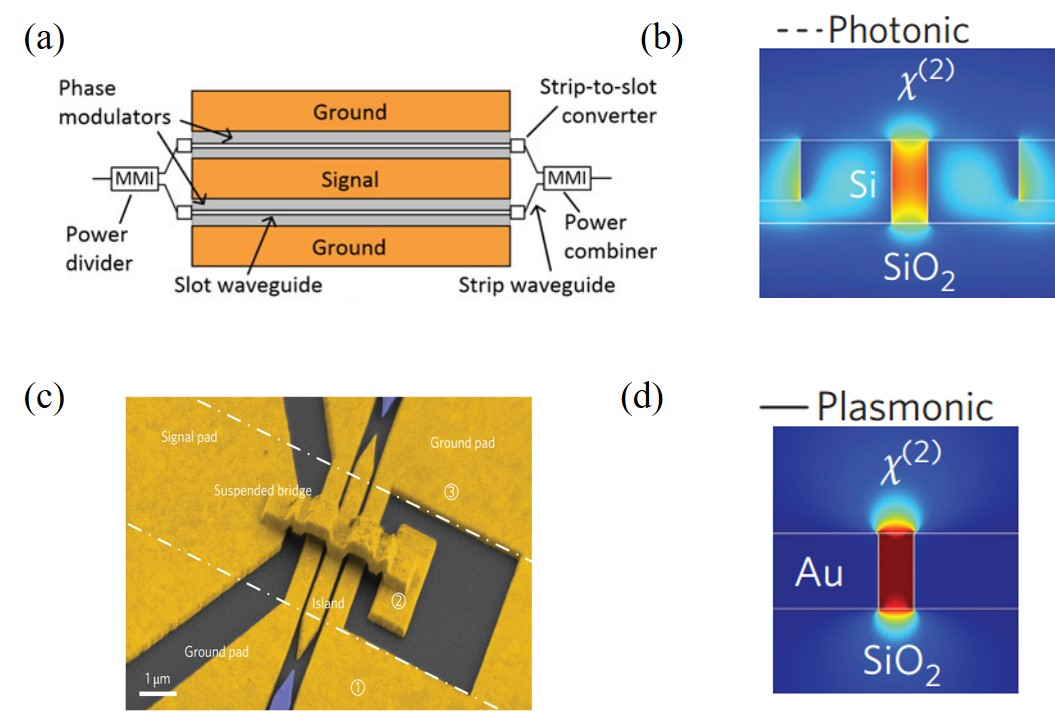
\includegraphics[width=12cm]{./Pictures/fig_polymer_mod.jpg}
	\caption{ (a) 硅基聚合物光调制器结构图\cite{palmer2014high};(b)硅基槽型波导模场分布\cite{palmer2014high};(c)硅基基于表面等离子体槽型波导聚合物型光调制器结构图\cite{haffner2015all};(d)硅基槽型表面等离子体波导模场分布图\cite{haffner2015all}}
	\label{fig_polymer_mod}
\end{figure}

\subsection{硅基其他电光材料光调制器}
目前主干网的光通信网络中,光调制器依旧大量采用铌酸锂(LiNbO3)光调制器。因此,很多研究人员尝试将铌酸锂等高电光系数的固体材料集成到硅平台上。表\ref{sil_others_mod}展示了最近将铌酸锂和钛酸钡(BaTiO3)薄膜混合集成到硅平台上,实现光调制器的性能。
{
	\begin{table}[htb]
		\zihao{5}
		\caption{硅基铌酸锂和钛酸钡的光调制器。}
		\label{sil_others_mod}
		\centering
		\begin{tabular}[t]{p{1.5cm}cp{1.2cm}ccccccc}
			\hline
			调制原理  & 电极结构 & 调制区尺寸 & 调制速度 & 动态能耗 & 消光比 & 插入损耗 & 调制电压\\
			\hline
			LiNbO3\cite{chen2014hybrid} & LE  & 30 $\mu m$ & 9 Gbps & 4.4 pJ/bit & 3 dB & 5 dB & 5 V\\
			BaTiO3\cite{xiong2014active} & LE  & 750 $\mu m$ & 300 Mbps & - & 3 dB & - & 6.6 V\\
			\hline
		\end{tabular}
	\end{table}
}
从表\ref{sil_others_mod}可以看出,这些材料的硅基光调制器性能还未完全开发。硅基铌酸锂光调制器采用铌酸锂薄膜放置到硅波导上表面,波导界面模场和器件结构图见图\ref{fig_othter_mod.jpg}(a,b)。这种光调制器最好的调制和能耗性能只有 9 Gbps和4.4 pJ/bit。最近高电光细数的钛酸钡被用于硅基光调制器,其电光系数达到了213 ± 49 pm/V \cite{xiong2014active},这种光调制器的结构和波导界面模场分布图如\ref{fig_othter_mod.jpg}(c-e)所示。虽然此光调制器速度目前只有 300 Mbps,通过合理设计电极仍然有提高的趋势。除此之外,压电陶瓷薄膜具有高电光系数(240 pm/V)也成功被溅射到了硅衬底上\cite{george2015lanthanide},这也是实现硅基新电光材料光调制器的新方案。未来将会有越来越多的新电光材料集成到硅平台上。
\begin{figure}[htb]
	\centering
	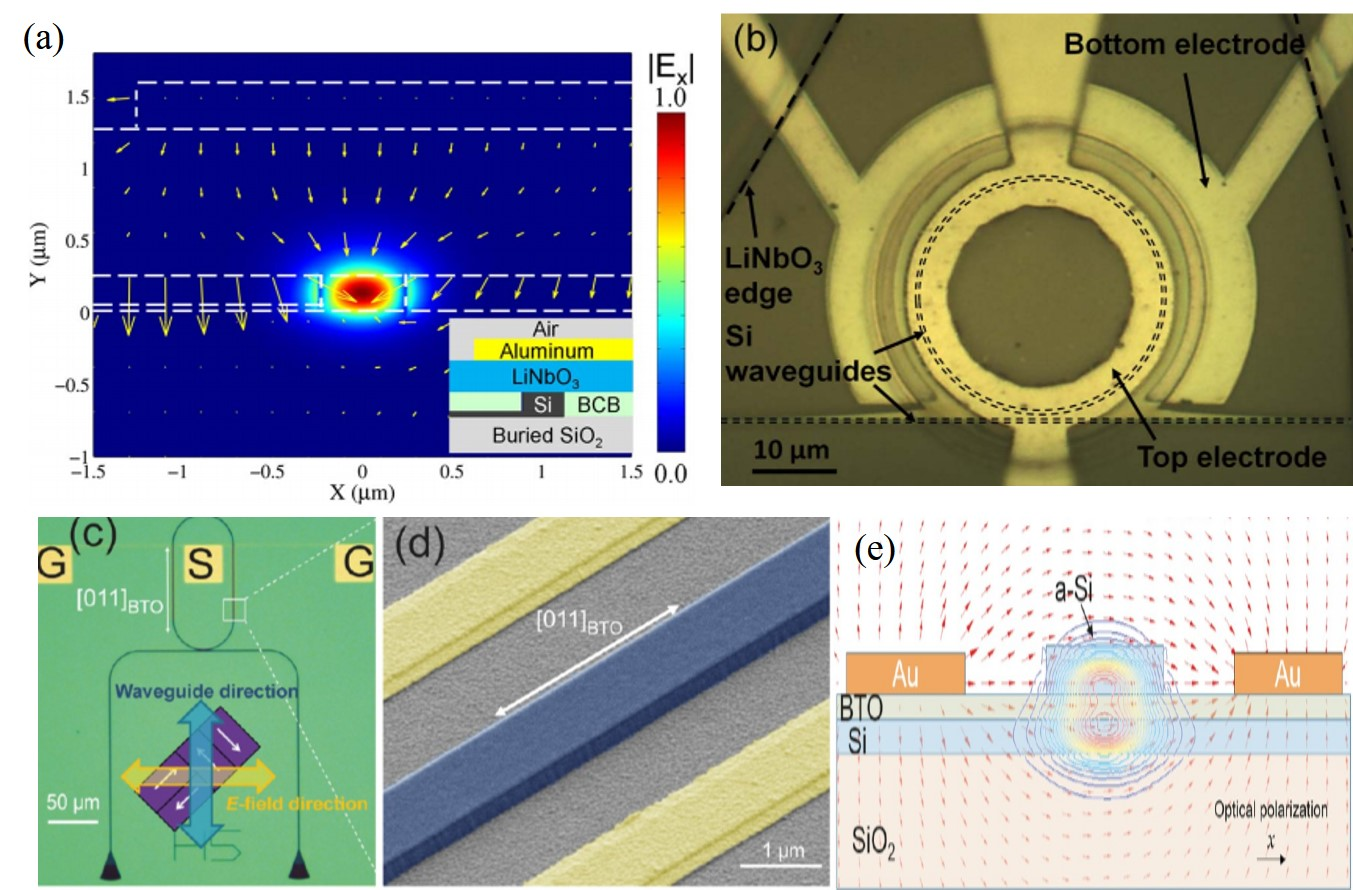
\includegraphics[width=12cm]{./Pictures/fig_othter_mod.jpg}
	\caption{ (a)硅基LiNbO3光调制器的截面和模场分布\cite{chen2014hybrid};(b)硅基LiNbO3光调器的俯视图\cite{palmer2014high};(c)硅基BaTiO3光调器的俯视图\cite{xiong2014active};(d)硅基BaTiO3光调器的局部放大图\cite{xiong2014active};(e)硅基BaTiO3光调器波导截面的模场分布图\cite{xiong2014active}}
	\label{fig_othter_mod.jpg}
\end{figure}
\subsection{硅基混合集成III-V光调制器}
自从1984年贝尔实验的研究人员发现了III-V量子阱中有强烈的量子束缚Stark效应(Quantum Confined Stark Effect, QCSE),可以实现电吸收调制器调\cite{miller1984band, wood1984high}。到如今, InP衬底的电吸收光调制器速度不仅达到了100 Gbps,并且与III-V激光器单片集成到了一起\cite{chacinski2009monolithically, kazmierski2009100}。另外根据Kramers-Kronig,材料折射率虚部的变化也会影响材料折射率实部,电吸收调制器不仅能做强度调制器,也能做相位调制器。文献[\citenum{poirier2015inp}]中,研究人员展示了单片集成III-V激光器和III-V相位调制器,实现了100 Gbps的双极化正交相移键控(Dual Polarization Quadrature Phase-Shift Keying, DP-QPSK)调制的发射器\cite{poirier2015inp}。 除此之外,高速电吸收调制器还有一个独特用处,可以同时作为高速探测器\cite{miller1985electric}。基于电吸收调制器这个特点,实现了单片集成的光收发模块\cite{welstand1996dual,chen2016wavelength},单片集成的光电光转化的微波发生器\cite{zhou2014compact}。

将III-V和Si混合集成在一起,一直是研究人员的梦想。可是III-V和Si的晶格具有8.1\%的不匹配程度,在Si上无法完美长出大面积III-V晶体。最近在硅基上虽然可以通过利用缓冲层和限制缺陷扩展的结构,外延生长InP的纳米线,实现了光泵浦激光器\cite{wang2015room},但是距离直接生长出III-V量子阱结构还差距很远。因此,目前是研究人员还是采用键合的方式将III-V和Si混合集成在一起,利用III-V直接带隙的特点,实现在硅基上电泵浦激光器,高速电吸收调制器,高速光探测器和半导体放大器\cite{liang2010hybrid,roelkens2010iii,liang2010recent,duan2014hybrid}。

\begin{figure}[htb]
	\centering
	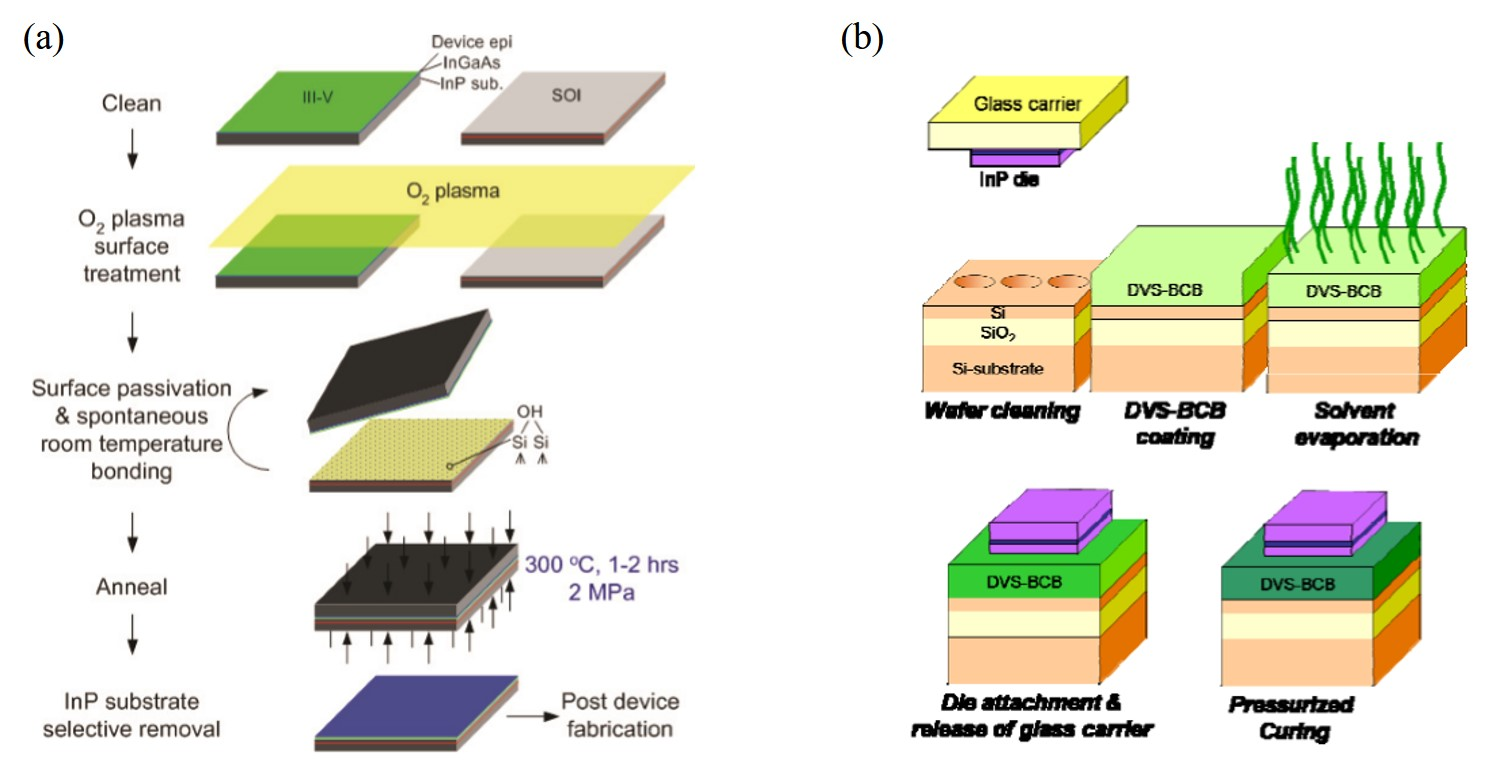
\includegraphics[width=14cm]{./Pictures/fig_bonding_methods.jpg}
	\caption{ (a) III-V和Si直接键合的工艺流程 \cite{liang2010hybrid, roelkens2010iii};(b) III-V和Si粘贴键合的工艺流程 \cite{liang2010hybrid, roelkens2010iii}}
\label{fig_bonding_methods}
\end{figure}

目前,有两种主流键合方式将III-V和Si混合集成在一起。第一种方式是III-V/Si直接键合,具体流程如图\ref{fig_bonding_methods}(a)所示。在III-V和Si键合表面先用氧等离子体分别活化,然后再将III-V和Si贴合,放置到300摄氏度的高压环境中退火。这种方法最早是瑞典的乌普萨拉大学的研究人员提出\cite{pasquariello2002plasma},而后经由美国加州大学圣塔芭芭拉分校的研究人员进一步优化\cite{liang2010hybrid},解决了键合表面产生气体的问题,不仅实现了第一个硅基混合集成的电泵浦III-V激光器\cite{fang2006electrically},也实现了第一个硅基混合集成的电吸收调制器\cite{kuo2008high}。第二种方式是III-V/SI粘贴键合,具体流程如图\ref{fig_bonding_methods}(b)所示。在III-V和Si表面中间添加一层粘贴剂,将它们紧密地键合在一起。虽然有很多种聚合物可以作为III-V和Si的粘贴剂,但是这种粘贴剂不仅不需要足够的粘贴强度,还需要厚度需要小于100 nm,便于光在硅波导和III-V波导之间的耦合。比利时根特大学的研究人员,利用稀释后的DVS-BCB(divinylsiloxane-bisbenzocyclobutene)聚合物实现了III-V和Si中间的粘贴层小于100nm\cite{liang2010hybrid, roelkens2010iii}。基于III-V/SI粘贴键合的混合集成平台上也同样实现了激光器,电吸收调制器等器件\cite{roelkens2015iii}。

\begin{figure}[htb]
	\centering
	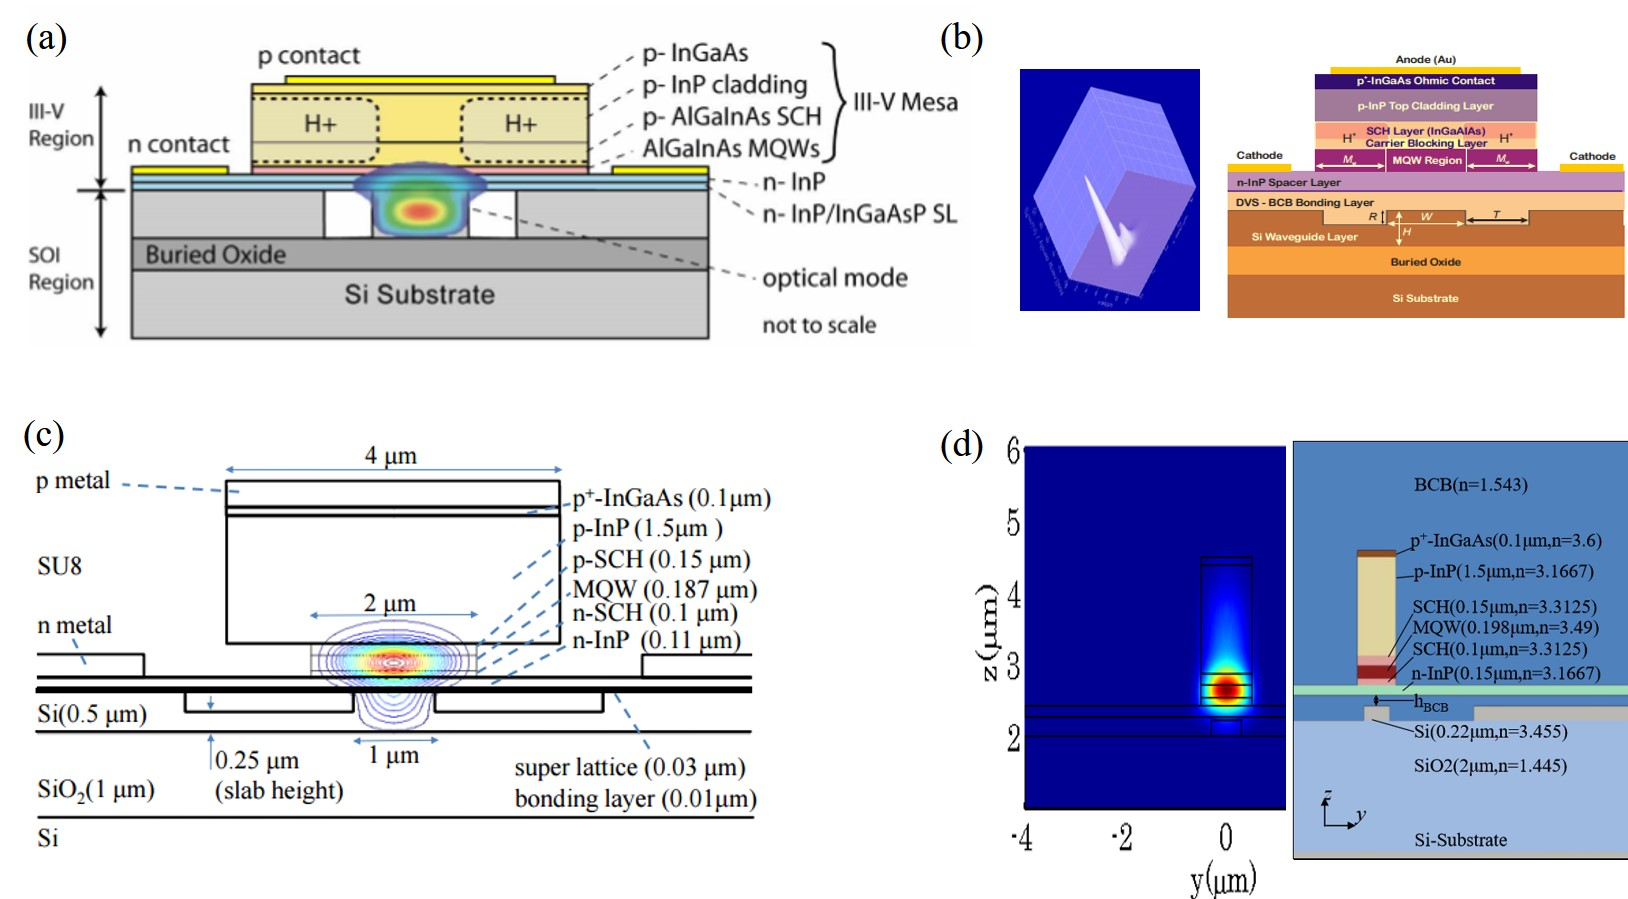
\includegraphics[width=12cm]{./Pictures/fig_hybrid_wg_cross.jpg}
	\caption{ (a) III-V/Si直接键合的混合集成波导截面结构和模场分布图\cite{fang2006electrically};(b) III-V/Si粘贴键合的混合波导模场分布图(左)和截面结构图(右)\cite{stankovic2010evanescently};(c) 用于调制器的III-V/Si直接键合的混合集成波导截面结构和模场分布图\cite{tang201150};(d) 用于调制器的III-V/Si粘贴键合的混合集成波导截面结构和模场分布图}
	\label{fig_hybrid_wg_cross}
\end{figure}

III-V/Si直接键合相比III-V/Si粘贴键合,III-V和Si之间的间隔更为紧密。图\ref{fig_hybrid_wg_cross}(a)展示了III-V/Si直接键合的混合集成波导截面结构和模场分布图,可以看到大部分光场集中在硅波导中,有部分倏逝波耦合到了III-V波导中。III-V/Si粘贴键合下,虽然他们之间的间隔相比而言比较远,但是由于粘贴剂的存在,对III-V和Si表面的粗糙度和洁净度容忍度更大\cite{gunther2007}。图\ref{fig_hybrid_wg_cross}(b)展示了III-V/Si粘贴键合的混合集成波导截面结构和模场分布图,光场也是大部分集中在硅波导中。不过,对于调制器而言,器件的尺寸越小,器件的电容就会越小,微波电极的损耗也越小,调制速度就会越快,因此需要将光大部分集中到III-V波导中,提高调制效率。图\ref{fig_hybrid_wg_cross}(b, c)分别展示了III-V/Si直接和粘贴键合平台下,调制器波导截面结构和模场分布图,可以两者结构中,通过减小硅波导的宽度,将光场大部分集中在III-V波导中,从而提高单位长度的调制效率,减少调制器尺寸。

硅基混合集成III-V光调制器自从2008年实现以后,性能逐年提高,电极种类囊括了图\ref{fig_mod_ele_type}中的四类,光学结构包含了图\ref{fig_mod_opt_type}中的三类。从表\ref{sil_IIIV_mod}中可以看出,调制速度最快的是采用TW和STLE结构的,速度到了50 Gbps,并且STLE电极的电光调制3 dB带宽达到了74 GHz\cite{tang2012over},这个调制速度和纯硅基光调制器的调制速度相当。最小尺寸的硅基混合集成III-V光调制器是采用图\ref{fig_mod_opt_type}中的第四种结构,基于调制微环的损耗,从而调制谐振波长的光强。该器件的示意图和实际器件如图\ref{fig_eam_ring}所示\cite{Srinivasan2012micro}。它直径24 $\mu m$的尺寸与纯硅基光调制器相比,还是偏大。在表中,我们也增加了自己最近的研究成果,实现了驱动电压只要50 mV, 动态功耗0.29 fJ/bit的电吸收光调制器。这种低驱动电压,低能耗的硅基混合集成III-V光调制器是目前所有光调制器中,驱动电压最低一类,并且在同样最低驱动电压下,实现了目前最大的消光比。除此之外,硅基混合集成的III-V电吸收调制器具有双工作模式,可以作为高速光探测器。凭借电吸收调制器的这种特性,我们展示了单片集成的光收发模块\cite{chen2016wavelength}。
{
	\begin{table}[htb]
		\zihao{5}
		\caption{硅基混合集成III-V光调制器研究进程。}
		\label{sil_IIIV_mod}
		\centering
		\begin{tabular}[t]{p{2cm}p{1cm}p{1cm}p{1.2cm}cccp{1cm}c}
			\hline
			键合方式  & \tabincell{c}{工作 \\ 方式} &\tabincell{c}{电极 \\ 结构}  & \tabincell{c}{调制区 \\ 尺寸} & 调制速度 & 动态能耗 & 消光比 & \tabincell{c}{插入 \\ 损耗} & 调制电压\\
			\hline
			直接键合\cite{kuo2008high} & EAM & LE & 250 $\mu m$ & 10 Gbps & - & 10 dB & 3 dB & 0.82 V\\
			直接键合\cite{tang201150} & EAM & TW & 100 $\mu m$ & 50 Gbps & 400 fJ/bit & 8.8 dB & 5 dB & 2 V\\
			直接键合\cite{tang2012over} & EAM & STLE & 100 $\mu m$ & 50 Gbps & 484 fJ/bit & 9.6 dB & 5 dB & 6.6 V\\
			直接键合\cite{tang2012energy} & EAM & LE & 100 $\mu m$ & 40 Gbps & 20 fJ/bit & 5 dB & 9 dB & 0.5 V\\
			直接键合\cite{chen2011forty} & EOM & CLTWE & 500 $\mu m$ & 40 Gbps & - & 6 dB & 9 dB & 4 V\\
			直接键合\cite{Srinivasan2012micro} & \tabincell{c}{EOM\\(Ring)} & LE & 24 $\mu m$ & - & 60 fJ/bit & - & - & 4 V\\
			粘贴键合\cite{fu20155} & EAM & LE  & 100 $\mu m$ & 28 Gbps & 200 fJ/bit & 5 dB & 1.2 dB & 2.4 V\\
			\tabincell{c}{粘贴键合 \\ (本论文工作)} & EAM & LE  & 80 $\mu m$ & 1.25 Gbps & 0.29 fJ/bit & 6.3 dB & 5 dB & 0.05 V\\
			\hline
		\end{tabular}
	\end{table}
}

\begin{figure}[htb]
	\centering
	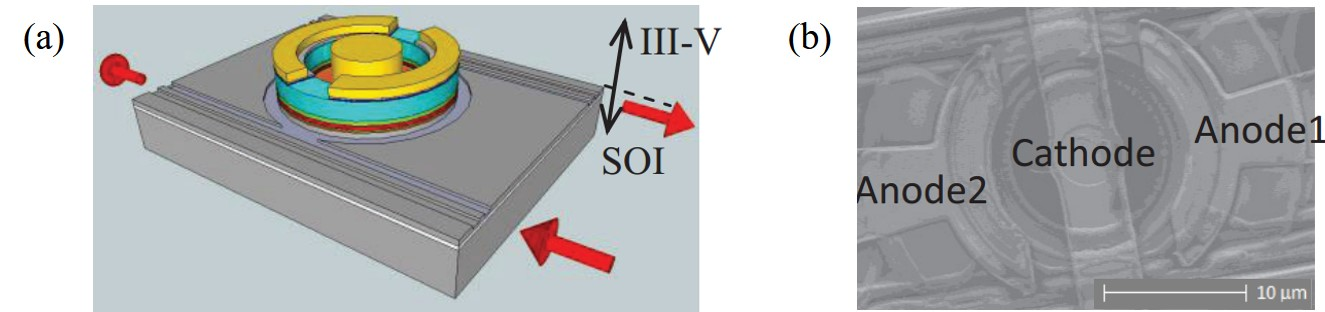
\includegraphics[width=12cm]{./Pictures/fig_eam_ring.jpg}
	\caption{ (a, b) 硅基混合集成III-V微环型光调制器的结构示意图和器件实际图\cite{Srinivasan2012micro}}
	\label{fig_eam_ring}
\end{figure}

\section{本论文的内容和创新点}
本论文主要分析讨论两种硅基光调制器。第一种是硅基混合集成III-V电吸收光调制器,第二种是纯硅基光调制器。对于第一种电吸收光调制器,我们的目标是降低驱动电压,减小能耗,缩小尺寸,以便提升器件的集成度,为日后半导体驱动电路和光器件单片集成提供基础。接着,我们充分利用电吸收调制器双工作模式,即调制器也可以作为高速探测器的特点,结合硅基无源器件,尝试在单个硅片上构建包含波分复用系统的光收发模块。对于第二种纯硅基光调制器,我们的目标是设计拥有新型光学结构的光调制器,实现在拥有大的光学带宽的同时,保持小的调制区域尺寸。

\subsection{本论文的章节安排}
第一章首先总结了硅基光电子集成技术的发展历史,以及目前最新的发展状况。然后着重介绍了硅基光调制器的性能指标,以及目前实现硅基光调制器的光学结构和电极结构。随后详细介绍了硅基上利用不同材料实现光调制器的原理,发展现状,性能指标,以及他们的优缺点。

第二章介绍了硅基混合集成III-V波导中两方面的设计。第一方面是量子阱结构的设计。首先介绍了用于电吸收光调制器量子阱结构的计算仿真方法,然后介绍了利用退火算法设计量子阱结构的思路。并且提供了利用退火算法设计偏振不敏感电吸收光调制器的量子阱结构的例子。第二方面是波导尺寸的设计,分析了混合集成III-V波导中矩形波导和蘑菇型波导尺寸的变化对光波和微波的影响,以及对调制速度的影响。

第三章介绍了硅基混合平台中,光从硅波导模式耦合到混合集成III-V波导模式的结构的设计。首先,我们分析了实现硅波导模式到混合集成III-V波导模式耦合的难点在于混合集成III-V波导中的高阶模式在耦合过程中容易被激发出来。为了解决这个问题,我们将耦合结构分成三个区域,逐渐将光耦合到最后的模式,从而减少激发出高阶模式。我们利用三维时域有限元差分(3D FDTD)的方法分别优化三个区域的耦合结构。接着,我们将优化后的三个区域组合成最终结构。整体结构的仿真结果,我们分别采用了3D FDTD和本征模式展开发(Eigenmode Expansion, EME)进行验证,并且比较了两种仿真方法的优缺点。最后,我们设计了用电子束曝光机制作这种紧凑耦合结构的方案。

第四章介绍了硅基混合集成III-V光调制器的研制。首先仿真计算了能带填充效应对量子阱激子吸收峰的影响和基于这种现象的电吸收调制器的性能。然后,我们详细介绍了制作硅基混合集成III-V光调制器的工艺步骤。接着,在搭建的测试光调制器的高速平台上,对其进高速性能的测试。 最后,我们测试还分析同个电吸收调制器在行波电极和集总电极两种工作模式下性能的区别。

第五章介绍了硅基混合集成III-V光调制器同时作为高速光探测器的性能。我们同样其进行高速性能测试,以及在高反向电压下雪崩现象的测试。接着,我们展示了单片混合集成整列波导光栅,6个高速调制器,6个高速探测器的的光收发模块的测试结果。

第六章介绍了基于可调反射镜和微环结构的新型纯硅基光调制器。首先,介绍了可调反射镜的工作原理。然后分析了微环内部反射率对微环透射谱的影响。最后分析了新型纯硅基光调制器的工作性能。

第七章总结了本论文的内容的,并且也对后期的工作和未来的硅基光调制器的发展方向进行了讨论和展望。

\subsection{本论文的主要创新点}
本论文利用快速退火算法,简化了设计III-V量子阱结构多参数的问题。我们进一步展示了通过合理设计权值函数,可以设计用于偏振不敏感电吸收光调制器的量子阱结构的例子。

本论文设计了紧凑的硅波导和混合集成III-V波导的光耦合结构。该结构是基于220 nm厚的SOI平台,利用III-V波导中3段锥形结构(Taper),将硅波导中的光缓慢地耦合到混合集成III-V波导中,从而降低在混合集成III-V波导中高阶模式的激发,从而实现长度只有8 $\mu m$的耦合结构,是目前文献报道中最紧凑的耦合结构。这个耦合结构的光学带宽具有100 nm以上,耦合效率都达到了95\%。我们也设计了用电子束曝光机制作这种紧凑耦合结构的方案。

本论文设计,制作,测试了硅基混合集成III-V电吸收光调制器,并且在世界上首次利用能带填充效应下量子阱中激子吸收峰的漂移,实现电吸收光调制器。第一次实现了电吸收光调制器在80  $\mu$m的长度下,驱动电压值只需要50 mV,动态能耗只有0.29 fJ/bit,于此同时,动态消光达到6.3 dB,调制速率达到1.25 Gbps。基于能带填充效应的电吸收调制器给了一种设计低驱动电压,低功耗,小尺寸的调制器的全新思路。另外,我们分析比较了同个电吸收调制器在行波电极和集总电极两种工作模式下性能的区别。

本论文借助于电吸收调制器在反偏电时既是调制器也是探测器的双工作状态的特点,在世界上首次展示了集成两个级联的整列波导光栅,6个高速调制器,6个高速探测器的单片硅基混合集成的光收发模块。信道的频率间隔是200 GHz,单个信道的收发传输速率达到30 Gbps。 在1.5 $\times$ 0.25 mm\SP{2} 的硅基芯片,利用混合集成技术上实现了 180 Gbps的光收发模块。除此之外,我们还详细介绍了通过优化工艺,能将单个电吸收调制器的速度能提高到40 Gbps。

最后,本论文首次提出了基于可调反射镜和微环结构的新型纯硅基光调制器。我们利用微环的透射谱对其内部反射率敏感的特点,通过在微环中引入片上集成的可调反射镜,通过调制可调反射镜的反射率,实现了输出光强度的调制。这种光调制器既有马赫-曾德尔光调制器大光学带宽的特点,也有微环调制器结构紧凑的特点。该设计的调制器相位调制区域只有20 $\mu$m,驱动电压只需要2 V,3 dB调制带宽将达到40 GHz。这种新结构不仅可以用于纯硅基光调制器,也可以用于硅基其他电光材料的光调制器。




